\documentclass[conference,compsoc]{IEEEtran}

\ifCLASSOPTIONcompsoc
  \usepackage[nocompress]{cite}
\else
  \usepackage{cite}
\fi

\ifCLASSINFOpdf

\else

\fi

\usepackage{tikz}
\usetikzlibrary{arrows.meta}
\definecolor{ink}{HTML}{202934}
\definecolor{blue}{HTML}{214E78}
\definecolor{green}{HTML}{285C4C}
\definecolor{gray}{HTML}{737B82}

\usepackage{xurl}
\usepackage{hyperref}
\hypersetup{hidelinks}



\usepackage{color}
\definecolor{revcolor}{rgb}{0,0.45,0.40}
\newcommand{\rev}[1]{#1} % revision marks neutralized for submission
\usepackage{amsmath}
\usepackage{amssymb}
\usepackage{graphicx}
\usepackage{placeins}
\usepackage{algorithm}
\usepackage{algpseudocode}
\hypersetup{hypertexnames=false}

\newif\ifcamera\camerafalse % S&P: Ethics section is camera-ready only; GenAI use goes in the HotCRP field
\newcommand{\sys}{Sluice}
\newcommand{\GviiiExecutionID}{\texttt{sluice-agentdojo-g8-\allowbreak
20260828-\allowbreak 23f31810\allowbreak 01cb404f\allowbreak
b7641c37\allowbreak e431a771}}
\newcommand{\GviiiManifestSHA}{\texttt{74302265\allowbreak b3dd9b21\allowbreak
68652630\allowbreak b03e754f\allowbreak d21872a5\allowbreak
d2ad899c\allowbreak 73558ec9\allowbreak 8cd6c5c3}}
% Auto-generated by generate_rq1_macros.py from a raw RQ1 results
% JSON. Do not hand-edit; regenerate instead.
\newcommand{\rqOneNCases}{25}
\newcommand{\rqOneNAttacks}{15}
\newcommand{\rqOneNControls}{10}
\newcommand{\rqOneUndefendedAttackSuccess}{15/15}
\newcommand{\rqOneSluiceAttackSuccess}{0/15}
\newcommand{\rqOneUndefendedOverallCompletion}{10/25}
\newcommand{\rqOneSluiceOverallCompletion}{25/25}
\newcommand{\rqOneSluiceCleanCompletion}{10/10}
\newcommand{\rqOneSluiceAttackedCompletion}{15/15}
\newcommand{\rqOneUndefendedAttackedCompletion}{0/15}

% Generated from authenticated C4 journals; do not edit.
\newcommand{\CFourHFourDelta}{-1.15\%}
\newcommand{\CFourHFourCILow}{-1.94\%}
\newcommand{\CFourHFourCIHigh}{-0.52\%}
\newcommand{\CFourHFourExecutionAdverseCIHigh}{-0.19\%}
\newcommand{\CFourHFourFallbackAdverseCIHigh}{0.58\%}
\newcommand{\CFourHFiveDelta}{-0.48\%}
\newcommand{\CFourHFiveCILow}{-1.22\%}
\newcommand{\CFourHFiveCIHigh}{0.19\%}
\newcommand{\CFourHFiveAdverseCILow}{-1.44\%}
\newcommand{\CFourErroredArms}{87}
\newcommand{\CFourAuthoringFallbackTasks}{15}
\newcommand{\CFourAuthoringFallbackGovernedArms}{225}
\newcommand{\CFourAuthoringFallbackHFourArms}{210}
\newcommand{\CFourAuthoringFallbackHFiveArms}{15}
\newcommand{\CFourAuthoringFallbackDevelopmentArms}{0}
\newcommand{\CFourFallbackBreakdownRows}{%
\texttt{granite31-8b} & 104729 & \texttt{workspace} & \texttt{user\_task\_38} & \texttt{heldout} & 1 & 15 \\
\texttt{granite31-8b} & 104729 & \texttt{workspace} & \texttt{user\_task\_26} & \texttt{heldout} & 1 & 15 \\
\texttt{granite31-8b} & 104729 & \texttt{workspace} & \texttt{user\_task\_35} & \texttt{heldout} & 1 & 15 \\
\texttt{granite31-8b} & 130363 & \texttt{workspace} & \texttt{user\_task\_26} & \texttt{heldout} & 1 & 15 \\
\texttt{granite31-8b} & 130363 & \texttt{workspace} & \texttt{user\_task\_35} & \texttt{heldout} & 1 & 15 \\
\texttt{granite31-8b} & 155921 & \texttt{workspace} & \texttt{user\_task\_26} & \texttt{heldout} & 1 & 15 \\
\texttt{granite31-8b} & 155921 & \texttt{workspace} & \texttt{user\_task\_35} & \texttt{heldout} & 1 & 15 \\
\texttt{granite31-8b} & 196613 & \texttt{workspace} & \texttt{user\_task\_27} & \texttt{heldout} & 1 & 15 \\
\texttt{granite31-8b} & 196613 & \texttt{workspace} & \texttt{user\_task\_38} & \texttt{heldout} & 1 & 15 \\
\texttt{granite31-8b} & 196613 & \texttt{workspace} & \texttt{user\_task\_26} & \texttt{heldout} & 1 & 15 \\
\texttt{granite31-8b} & 196613 & \texttt{workspace} & \texttt{user\_task\_35} & \texttt{heldout} & 1 & 15 \\
\texttt{granite31-8b} & 262147 & \texttt{workspace} & \texttt{user\_task\_38} & \texttt{heldout} & 1 & 15 \\
\texttt{granite31-8b} & 262147 & \texttt{workspace} & \texttt{user\_task\_26} & \texttt{heldout} & 1 & 15 \\
\texttt{granite31-8b} & 262147 & \texttt{workspace} & \texttt{user\_task\_35} & \texttt{heldout} & 1 & 15 \\
\texttt{qwen25-3b} & 196613 & \texttt{workspace} & \texttt{user\_task\_38} & \texttt{heldout} & 1 & 15 \\
}





\begin{document}

\title{Sluice: Capability-Based Mediation with Conditional Information-Flow Bounds for LLM Agents}


\author{Anonymous Submission}





\maketitle


\begin{abstract}
\rev{
LLM-agent workflows need controls over both confidential releases and actions influenced by untrusted input. \sys{} is a capability-based mediation library that combines finite typed gates, atomic integer budget reservation before backend decoding, and one-time, effect-scoped action capabilities. Its \textsc{Release} gates support a conditional confidentiality bound; its \textsc{Endorse} gates constrain authorized effects without an information-theoretic integrity guarantee.

For a single protected object and policy epoch, we prove that the mutual information in a finite, non-timing-typed transcript is at most the configured budget $B$. Under the same premises, the adversary's guessing advantage grows by at most a factor of $2^{B}$, and $m$ objects leak at most the sum of their caps. The premises carry the weight: the secret must not reach the caller, and routing, request metadata, denials, and post-result metadata must be secret-independent. A counterexample shows that charging gate selection only after a successful claim cannot protect secret-dependent routing. The TLC model checker verified ledger and sequencing safety over 184{,}016 distinct states of the bounded TLA\textsuperscript{+} model.

We evaluate with exhaustive synthetic leakage experiments, regression and workflow attack tests, and a prospectively frozen AgentDojo study of the \textsc{Endorse} direction (31{,}380 arms, three open-weight models, five seeds). On this fixed corpus, \sys{} lowers macro-averaged attack success from 1.81\% to 0.66\% (difference $-1.15$ percentage points; 95\% CI $[-1.94,-0.52]$) and meets a prespecified five-point supported-utility non-inferiority margin ($\Delta=-0.48$; 95\% CI $[-1.22,0.19]$). The effect is concentrated in one 3B model, an adverse sensitivity analysis for policy-authoring fallbacks crosses zero, and the comparator is weak.
}
\end{abstract}

\begin{IEEEkeywords}
LLM agent security, quantitative information flow, capability-based access control, reference monitors, prompt injection, formal verification.
\end{IEEEkeywords}





\IEEEpeerreviewmaketitle



\section{Introduction}
\label{sec:intro}

Autonomous LLM agents compose retrieval, tool use, and delegation into
workflows with external effects. Such workflows mix protected content,
attacker-controlled content, model outputs, and tool arguments. These induce
different security questions. A \textsc{Release} mechanism may bound what a
secret reveals to a stated observer; an \textsc{Endorse} mechanism may
constrain effects chosen after untrusted input, but a confidentiality lemma
does not become an integrity theorem by renaming the input.

\rev{\paragraph{Scope} Recent attacks and surveys show that both directions are exercised in practice~\cite{sokagentic2026,masleak2026}. A finite trusted-authored alphabet with a $\log_2 K$-bit cost per call, summed over calls, is the obvious starting point. It is not enough alone: (1) the per-call bound is an elementary consequence of $I(X;Y)\le H(Y)\le\log_2|\mathrm{supp}(Y)|$; (2) OCELOT~\cite{ocelot2026} and MNC~\cite{mnc2026} (\S\ref{sec:related}) already implement overlapping mechanisms; and (3) an independent-call argument does not cover interactive traces whose later queries depend on earlier observations. \sys{} contributes the pieces below and keeps implemented mechanisms, proofs, model-checked properties, and measurements separate (Table~\ref{tab:claims}).}

\paragraph{Contributions}
\begin{itemize}
\item \textbf{Formal.} \rev{A conditional chain-rule bound for a finite, non-timing \textsc{Release} transcript whose premises enumerate the observer view (routing, request and authentication metadata, denials, typed results, capability and effect metadata, stopping, reauthorization), with guessing-advantage and multi-object corollaries (\S\ref{sec:proof}). A counterexample shows why charging selection only on successful claims cannot cover secret-dependent routes. TLC checks the bounded TLA\textsuperscript{+} model for atomic claim-and-reserve, spending within the budget cap, and mutually exclusive successor claims.}
\item \textbf{System.} \rev{A reference-monitor API with no caller parameter for the alphabet, cost, protected object, or provenance; atomic reserve-before-decode integer accounting with zero overshoot by construction; optionally redeemer-bound one-time action capabilities (\S\ref{sec:design}); and opt-in agent-identity authentication with single-hop delegation. The credential authenticates a request's origin, not a live channel-bound presenter (\S\ref{sec:tcb}, \S\ref{sec:multiagent}).}
\item \textbf{Empirical.} \rev{Exact enumeration of synthetic single- and two-object channels, including a scheduler that branches on prior public outcomes; regression and workflow attack suites; absolute latency; and a prospectively frozen AgentDojo study (G8, 31{,}380 arms) of the \textsc{Endorse} direction. The first AgentDojo run was invalidated by audit and two replacements failed closed; we report that history in Appendix~\ref{app:rq6-audit}. RQ1, RQ5, and RQ7 are illustrative (\S\ref{sec:eval}).}
\end{itemize}

\begin{table*}[t]
\centering
\caption{\rev{Claims, the assumptions they need, and the evidence behind them.}}
\label{tab:claims}
\rev{\footnotesize
\begin{tabular}{p{0.19\textwidth}p{0.26\textwidth}p{0.25\textwidth}p{0.19\textwidth}}
\hline
Claim & Assumptions & Evidence & Not claimed \\
\hline
Budget accounting, no overspend, successor exclusion & Integer ledger in one SQLite transaction & Regression tests; TLC, 184{,}016 states (\S\ref{sec:mechanization}) & Secret independence; timing \\
\textsc{Release} bound $I(S;T)\le B$ and corollaries & Premises 1--5: secret not visible to the caller, public schedule, no metadata channel, finite $N$ & Proof (\S\ref{sec:proof}); synthetic enumeration consistent with the bound (\S\ref{sec:eval}) & General enforcement of the premises; production confidentiality \\
Effect confinement by one-time capabilities & Calls routed through the monitor's executor & Tests and nine workflow attack cases (\S\ref{sec:eval}) & Complete mediation; same-process isolation \\
Request authentication and delegation & Per-agent HMAC keys held by the monitor & Credential and delegation tests (\S\ref{sec:multiagent}) & Channel-bound possession; collusion \\
Attack-success reduction & Fixed corpus, three models, model-authored policies (\S\ref{sec:rq6}) & G8 study & Unseen models/corpora; per-model inference \\
\hline
\end{tabular}}
\end{table*}

\section{Threat Model}
\label{sec:threat}

\paragraph{Principals} A trusted planner $P$ authors gates from its own
policy. Agents and tools act as callers with a \texttt{caller\_id}, by
default authenticated by the integration layer (a stated TCB boundary,
\S\ref{sec:tcb}). A gate may instead opt into
\texttt{require\_authenticated\_caller} (\S\ref{sec:multiagent}), requiring
the monitor itself to verify a fresh, request-bound signature before
granting an identity claim any weight -- authenticating the request's
origin, not a live channel-bound presenter (\S\ref{sec:tcb}); delegation
across agent boundaries is verified the same way. The environment
supplies untrusted content:
retrieved documents, tool outputs, or another agent's message.

\paragraph{Two directions} \textsc{Release} gates bound the confidential
information a protected secret can convey to a less-trusted observer under
the theorem's assumptions. \textsc{Endorse} gates reuse the same finite gate,
budget, replay, and action-policy machinery for attacker-controlled input,
but this does not instantiate the confidentiality theorem or prove an
integrity metric; its defensible interpretation is budgeted mediated
decision bandwidth under an explicit effect policy.

\paragraph{Attacker capabilities and generality} The attacker controls
the content of any untrusted input reaching a gate, can choose an arbitrary
invocation pattern up to a separate public finite attempt horizon $N$ (the
prototype does not enforce this horizon), can attempt replay and
failure/timeout/retry paths, and may
know the complete design of \sys{} (no security through obscurity), but
does \emph{not} control the trusted planner's policy, the monitor's
signing key, or an authorizer's reauthorization key (modeled as
external to the monitor, \S\ref{sec:design}). This model is not tied to
one model family: it is exercised with LangGraph and five open-weight
models spanning five vendors. The AgentDojo history includes an invalidated
integration, two terminal fail-closed replacements, and a separate completed
G8 identity whose fixed-corpus results are reported with their sensitivity and
assay limitations (\S\ref{sec:rq6}). The attacker
requires no privileged access -- only the ability to place content into a
channel the agent
already treats as legitimate input, the ordinary operating condition of
any system that composes retrieval, tool use, or delegation. \rev{Indirect injection through retrieved content is documented in the wild~\cite{greshake2023,retrievalbarrier2026}, and tool telemetry is a further untrusted channel~\cite{aiops2026}.} The
RQ1 cases are deliberately constructed mechanism tests, not a random sample
of real attacks.

\paragraph{Trusted computing base}
\label{sec:tcb}
The \sys{} monitor process, its HMAC key, and -- for a gate that opts into
\texttt{require\_authenticated\_caller} -- the registry of per-agent keys
(\texttt{agent\_keys}, \S\ref{sec:multiagent}) supplied by trusted
deployment code, exactly like \texttt{trusted\_planner\_identities}
already is. What \texttt{CallerCredential} verification proves is
narrower than ``proof of possession'' in the live, channel-bound sense
that term usually carries: a fresh HMAC signature, bound to one gate,
workflow, epoch, content digest, and args digest, with a single-use
nonce and a short expiry, produced by \emph{some} process that held the
named agent's key \emph{at signing time}. Absent mTLS, authenticated IPC,
or OS peer credentials binding the credential to its channel -- none of
which this prototype implements -- the monitor cannot distinguish the
genuine key-holder's request from an exact copy relayed by whoever
captured it first: the single-use nonce is usable exactly once, by
whichever presenter reaches the monitor first, not necessarily the
key-holder. \S\ref{sec:multiagent}'s own attack suite demonstrates and
accepts this boundary rather than claiming to close it. The prototype can
persist the monitor's own HMAC key in the durable store for
restart/reproducibility tests; this does not protect against a database
writer, who instead requires an externally supplied key (e.g., a KMS)
held by an isolated broker. The Python backend adapter/runtime executes in
the monitor process and is therefore in the prototype TCB for containment:
validation cannot stop it from reading process memory, using ambient I/O, or
terminating the process. Only the model-supplied candidate is adversarial and
re-validated against the committed alphabet. A genuinely untrusted decoder
requires a restricted RPC/process boundary not implemented here.

\paragraph{Explicit non-goals} Timing side channels are out of scope. \rev{Network-level and metadata channels of deployed agents~\cite{netleak2026} are likewise outside the typed transcript unless an integration includes them in $A_i$ or $M_i$.} The
theorem also excludes secret-dependent caller identities, credentials or
digests, arguments, redeemer choices, capabilities, effects, and audit fields
unless they are represented in a charged finite alphabet. Complete mediation
of \emph{every} possible path
into an action (files, sockets, shared memory, a tool invoked directly
without going through the monitor) is a property of a specific,
integrated deployment, not of this library; \S\ref{sec:impl} reports what
one real integration actually achieves and where it does not.

\FloatBarrier
\section{Design}
\label{sec:design}








\begin{figure*}
    \centering
\resizebox{\textwidth}{!}{
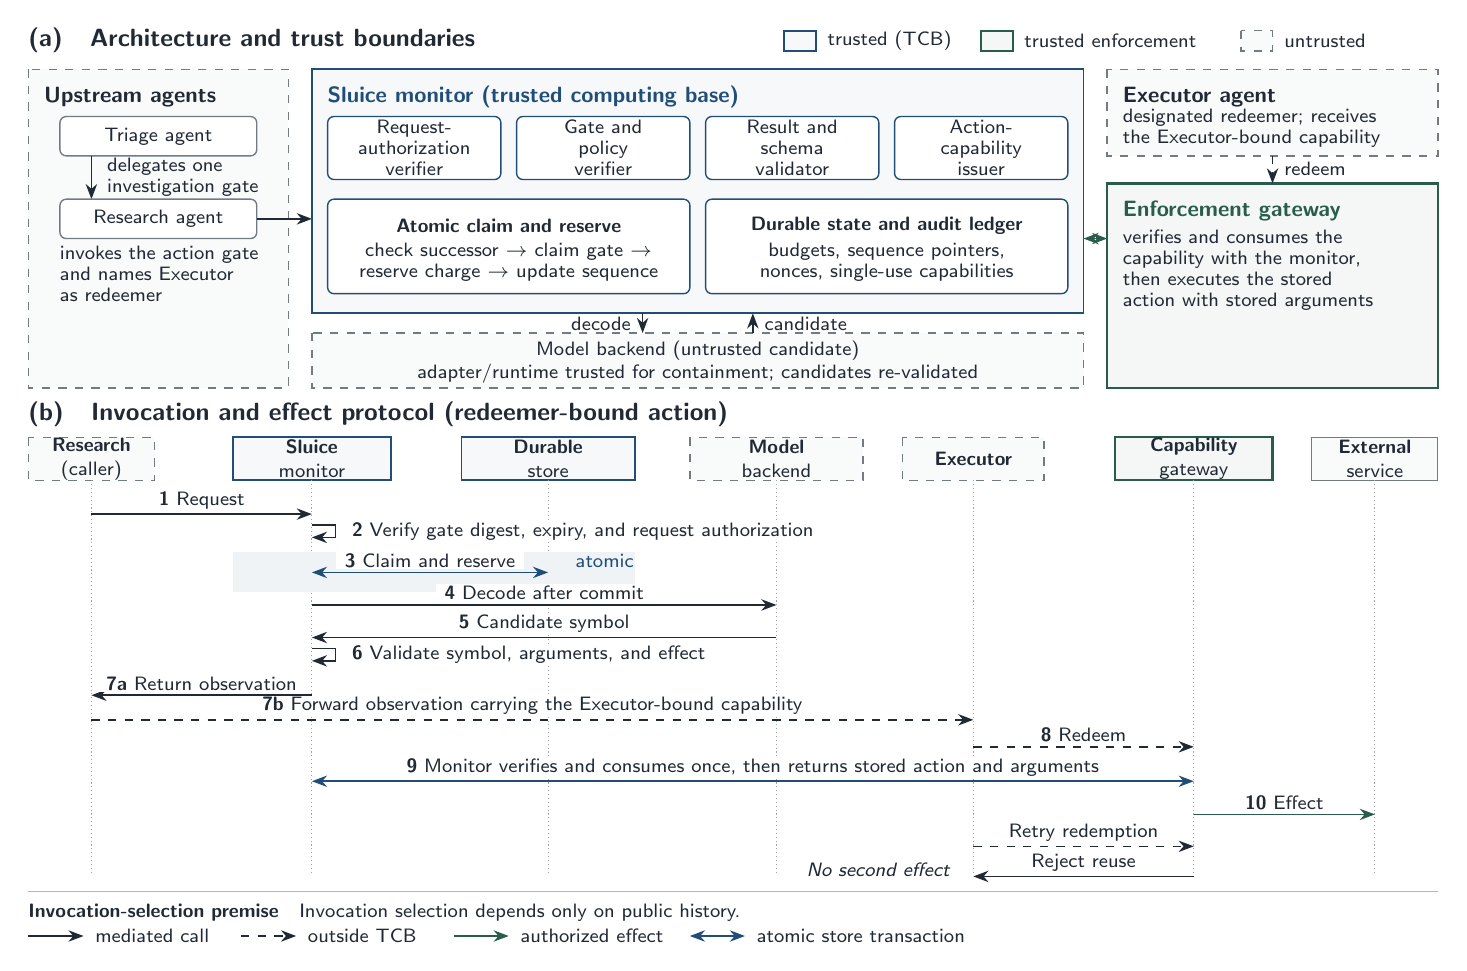
\begin{tikzpicture}[x=1mm,y=-1mm,font=\sffamily\fontsize{7.5}{8.7}\selectfont,
 text=ink,inner sep=0pt,outer sep=0pt,>=Stealth,
 heading/.style={anchor=west,font=\sffamily\bfseries\fontsize{9}{10}\selectfont},
 title/.style={anchor=west,font=\sffamily\bfseries\fontsize{8}{9}\selectfont},
 lefttxt/.style={anchor=west,align=left},
 tiny/.style={font=\sffamily\fontsize{6.6}{7.6}\selectfont},
 flow/.style={->,line width=.55pt,draw=ink},
 msg/.style={fill=white,inner xsep=1.1mm,inner ysep=.25mm},
 trust/.style={draw=blue,fill=blue!4,line width=.65pt},
 outside/.style={draw=gray,dashed,fill=gray!4,line width=.55pt},
 guard/.style={draw=green,fill=green!5,line width=.85pt},
 comp/.style={draw=blue,fill=white,rounded corners=.8mm,line width=.5pt},
 compg/.style={draw=gray,fill=white,rounded corners=.8mm,line width=.5pt}]
\node[heading] at (0,1.8) {(a)\quad Architecture and trust boundaries};
\draw[trust] (96,0.6) rectangle (100,3.2); \node[lefttxt,tiny] at (101.5,1.9) {trusted (TCB)};
\draw[guard] (121,0.6) rectangle (125,3.2); \node[lefttxt,tiny] at (126.5,1.9) {trusted enforcement};
\draw[outside] (154,0.6) rectangle (158,3.2); \node[lefttxt,tiny] at (159.5,1.9) {untrusted};
\draw[outside] (0,5.5) rectangle (33,46);
\node[title] at (2,9) {Upstream agents};
\draw[compg] (4,11.5) rectangle (29,16.5); \node[align=center] at (16.5,14) {Triage agent};
\draw[flow] (8,16.5)--(8,22);
\node[lefttxt,tiny] at (10,19.25) {delegates one\\investigation gate};
\draw[compg] (4,22) rectangle (29,27); \node[align=center] at (16.5,24.5) {Research agent};
\node[lefttxt,tiny] at (4,31.5) {invokes the action gate\\and names Executor\\as redeemer};
\draw[flow] (29,24.5)--(36,24.5);
\draw[trust] (36,5.5) rectangle (134,36.5);
\node[title,text=blue] at (38,9) {Sluice monitor (trusted computing base)};
\draw[comp] (38,11.5) rectangle (60,19.5);  \node[align=center,tiny] at (49,15.5) {Request-\\authorization\\verifier};
\draw[comp] (62,11.5) rectangle (84,19.5);  \node[align=center,tiny] at (73,15.5) {Gate and\\policy\\verifier};
\draw[comp] (86,11.5) rectangle (108,19.5); \node[align=center,tiny] at (97,15.5) {Result and\\schema\\validator};
\draw[comp] (110,11.5) rectangle (132,19.5);\node[align=center,tiny] at (121,15.5) {Action-\\capability\\issuer};
\draw[comp] (38,22) rectangle (84,34);
 \node[align=center] at (61,25.4) {\bfseries Atomic claim and reserve};
 \node[align=center,tiny] at (61,30) {check successor $\rightarrow$ claim gate $\rightarrow$\\reserve charge $\rightarrow$ update sequence};
\draw[comp] (86,22) rectangle (132,34);
 \node[align=center] at (109,25.4) {\bfseries Durable state and audit ledger};
 \node[align=center,tiny] at (109,30) {budgets, sequence pointers,\\nonces, single-use capabilities};
\draw[outside] (36,39) rectangle (134,46);
\node at (85,41.3) {Model backend (untrusted candidate)};
\node[tiny] at (85,44.2) {adapter/runtime trusted for containment; candidates re-validated};
\draw[flow] (78,36.5)--(78,39); \node[tiny,anchor=east] at (76.5,37.8) {decode};
\draw[flow] (92,39)--(92,36.5); \node[tiny,anchor=west] at (93.5,37.8) {candidate};
\draw[outside] (137,5.5) rectangle (179,16.5);
\node[title] at (139,9) {Executor agent};
\node[lefttxt,tiny] at (139,13) {designated redeemer; receives\\the Executor-bound capability};
\draw[guard] (137,20) rectangle (179,46);
\node[title,text=green] at (139,23.5) {Enforcement gateway};
\node[lefttxt,tiny] at (139,31) {verifies and consumes the\\capability with the monitor,\\then executes the stored\\action with stored arguments};
\draw[flow,dashed] (158,16.5)--(158,20); \node[tiny,anchor=west] at (159.5,18.2) {redeem};
\draw[flow,<->,draw=green] (134,27)--(137,27);
\begin{scope}[shift={(0,46)},y=-.78mm]\begin{scope}[shift={(0,-46)}]
\node[heading] at (0,50.3) {(b)\quad Invocation and effect protocol (redeemer-bound action)};
\newcommand{\participant}[4]{\draw[#3] (#1-#2,54) rectangle (#1+#2,61);
 \node[align=center] at (#1,57.5) {\bfseries #4};
 \draw[gray!70,densely dotted] (#1,61)--(#1,125);}
\participant{8}{8}{outside}{Research\\(caller)}
\participant{36}{10}{trust}{Sluice\\monitor}
\participant{66}{11}{trust}{Durable\\store}
\participant{95}{11}{outside}{Model\\backend}
\participant{120}{9}{outside}{Executor}
\participant{148}{10}{guard}{Capability\\gateway}
\participant{171}{8}{draw=gray,fill=gray!4}{External\\service}
\fill[blue!7] (26,72.6) rectangle (77,79.2);
\node[anchor=west,tiny,text=blue] at (69.5,74.2) {atomic};
\newcommand{\messagearrow}[5][]{\draw[flow,#1] (#2,#4)--(#3,#4)
 node[midway,above=.4mm,msg]{#5};}
\newcommand{\localcheck}[2]{\draw[flow] (36,#1)--(39,#1)--(39,#1+2)--(36,#1+2);
 \node[anchor=west,msg] at (40,#1+1) {#2};}
\messagearrow{8}{36}{66.5}{\textbf{1} Request}
\localcheck{68.3}{\textbf{2} Verify gate digest, expiry, and request authorization}
\messagearrow[<->,draw=blue]{36}{66}{76}{\textbf{3} Claim and reserve}
\messagearrow{36}{95}{81.3}{\textbf{4} Decode after commit}
\messagearrow{95}{36}{86.6}{\textbf{5} Candidate symbol}
\localcheck{88.4}{\textbf{6} Validate symbol, arguments, and effect}
\messagearrow{36}{8}{96}{\textbf{7a} Return observation}
\messagearrow[dashed]{8}{120}{100}{\textbf{7b} Forward observation carrying the Executor-bound capability}
\messagearrow[dashed]{120}{148}{104.4}{\textbf{8} Redeem}
\messagearrow[<->,draw=blue]{148}{36}{110}{\textbf{9} Monitor verifies and consumes once, then returns stored action and arguments}
\messagearrow[draw=green]{148}{171}{115.4}{\textbf{10} Effect}
\messagearrow[dashed]{120}{148}{120.6}{Retry redemption}
\messagearrow{148}{120}{125.5}{Reject reuse}
\node[anchor=east,font=\sffamily\itshape\fontsize{7.5}{8.7}\selectfont] at (117,124.4) {No second effect};
\draw[gray!55] (0,128)--(179,128);
\node[lefttxt] at (0,131.4) {\textbf{Invocation-selection premise}\quad Invocation selection depends only on public history.};
\draw[flow] (0,135.2)--(7,135.2); \node[lefttxt,tiny] at (8.5,135.2) {mediated call};
\draw[flow,dashed] (27,135.2)--(34,135.2); \node[lefttxt,tiny] at (35.5,135.2) {outside TCB};
\draw[flow,draw=green] (54,135.2)--(61,135.2); \node[lefttxt,tiny] at (62.5,135.2) {authorized effect};
\draw[flow,<->,draw=blue] (84,135.2)--(91,135.2); \node[lefttxt,tiny] at (92.5,135.2) {atomic store transaction};
\end{scope}
\end{scope}
\end{tikzpicture}
}
\caption{Sluice's architecture and invocation protocol. (a) The trusted monitor (blue) verifies requests and gate policy, atomically claims gates and reserves budget in the durable store, validates model results and proposed actions, and issues single-use capabilities. The upstream agents and their delegation requests lie outside the monitor's trust boundary. The same-process backend adapter/runtime is trusted for containment. The monitor checks each model-supplied candidate against the alphabet in the verified gate record. (b) In the redeemer-bound workflow (\S\ref{sec:multiagent}), the monitor commits the budget reservation (step~3) before the backend decodes the content (step~4). It then validates the candidate symbol, action arguments, and permitted effect (step~6). On success, the monitor returns an observation carrying a capability bound to Executor (step~7a), and Research forwards that observation to Executor (step~7b). Executor requests redemption through the trusted enforcement gateway (green, step~8). The monitor verifies the redeemer credential, consumes the capability, and returns the stored action and arguments (step~9). The gateway executes that action with those arguments (step~10). A replay after successful redemption is rejected before a second effect can occur.}
\label{fig:architecture}
\end{figure*}






\subsection{Capability-based API}
The caller-facing surface is exactly one method:
\texttt{invoke(handle, content, caller\_id, args=None)}. \texttt{handle} is an opaque
\texttt{(gate\_id, digest)} pair; the monitor resolves it against an
internally stored, immutable \texttt{GateRecord} and independently
recomputes the digest before proceeding. No caller-facing method accepts
an alphabet, cardinality, cost, protected-object name, or provenance
assertion (verified structurally, not just by convention: the
\texttt{invoke} signature literally has no such parameter,
\S\ref{sec:eval}). {Alg.~\ref{alg:invoke} presents the invocation decision path, including authorization, budget reservation before backend decoding, result and action validation, and issuance of a one-time capability.}

\subsection{GateRecord and the observable alphabet}
A \texttt{GateRecord} is created only by \texttt{author\_gate()}, called
by the trusted planner, and binds: a finite symbol set with
trusted-authored \texttt{ActionTemplate}s, a fixed integer charge
$\widehat c=\lceil 10^6\log_2(K+4)\rceil$ microbits computed by the
monitor (never accepted from a caller, so it is structurally impossible
for a caller to supply a negative, NaN, or infinite cost), a
permitted-caller set, an expiration, and an HMAC-SHA256 digest over an
exact-UTF-8, length-prefixed encoding of all of the above. Policy
strings are rejected unless already in NFC; the encoder never
normalizes two runtime-distinct strings to the same authenticated value.
The charged support contains the $K$ typed \texttt{OK} symbols plus
\texttt{SCHEMA\_VIOLATION}, \texttt{BACKEND\_ERROR},
\texttt{ARG\_INVALID}, and \texttt{EFFECT\_TOO\_STRONG}. Public pre-decode
rejections are outside that charged support only under the assumptions in
\S\ref{sec:proof}.

\subsection{Atomic reservation}
\texttt{invoke()} claims the one-time gate and reserves its full charge
against the protected object's budget \emph{before backend decoding},
inside one \texttt{BEGIN IMMEDIATE} transaction. The authoritative cap,
charge, and spend columns are integers: configured caps are rounded down to
microbits, gate costs are rounded up, and authorization uses exact integer
addition. If a reservation would exceed the cap, the backend is not called.
Optional credential verification recomputes SHA-256 digests from the submitted
content and arguments before this transaction: reserve-before-decode is not
reserve-before-any-read. Those digest values are visible fields of the
credential; its HMAC authenticates them but does not conceal them. A public
digest of a low-entropy secret permits offline dictionary testing. Therefore an
authenticated \textsc{Release} path satisfies the theorem only if the
credential channel and free authentication outcome are private or satisfy the
stated secret-independence premises (\S\ref{sec:proof}). Failed decoding is not
refunded.

\subsection{Successor sequencing and the selection charge}
\label{sec:sequencing}
The confidentiality theorem (\S\ref{sec:proof}) assumes a public adaptive
schedule: which gate is invoked next, and whether the caller stops, is a
function of the already-public typed transcript. It may depend on a prior
released result; it may not use an additional hidden view of the secret or
secret-dependent metadata omitted from that transcript.

The optional successor mechanism does not relax that premise. A
\texttt{GateRecord} may
declare \texttt{allowed\_successor\_gates}: the finite, authenticated set of
gate identifiers a caller may legitimately invoke immediately after this
one, for the same protected object and epoch. The first gate in a chain may
declare \texttt{entry\_fanout}: how many mutually exclusive entry points a
caller was choosing among before any gate in this chain was invoked. Both
fields are part of the authenticated, digest-bound \texttt{GateRecord}
format.

On \texttt{invoke()}, the monitor looks up the last successfully charged
gate for this (protected object, epoch) -- server-side state, never
supplied by the caller -- to determine the claim's fanout: its own
\texttt{entry\_fanout} if no predecessor is recorded and no other gate
reserves it as a successor, or the size of the recorded predecessor's
\texttt{allowed\_successor\_gates} otherwise, with anything outside that
declared set rejected charged zero (\texttt{UNAUTHORIZED\_SUCCESSOR}) --
a gate reserved as a declared successor may not also be claimed as a
free-standing entry point, which would otherwise let a caller skip its
predecessor and pay only its own \texttt{entry\_fanout}. If the fanout is
$\geq 2$, an additional $\lceil 10^6\log_2(\text{fanout})\rceil$
microbits are reserved atomically alongside the gate's own content
charge, before backend decoding -- the same worst-case-support logic
already used for the $K+4$ typed content charge, applied to gate
selection. A chain that never declares \texttt{allowed\_successor\_gates}
pays nothing extra and is never rejected by either check: the mechanism
is opt-in per chain. RQ3 and the TLA+ model exercise authorization and mutual
exclusion; workload measurements do not depend on it. Because denial reveals
the selected gate without reserving the fanout charge, secret-dependent
routing remains outside the theorem.

\subsection{Action templates}
A symbol may bind an \texttt{ActionTemplate}: a tool name, typed
argument constraints (allowed-value sets, regex patterns, or length
bounds; undeclared arguments are rejected by default, not silently
accepted), a recipient/resource scope, and a maximum effect class
(\texttt{none}/\texttt{reversible}/\texttt{irreversible}). Selecting a
symbol is necessary but not sufficient to act: \texttt{invoke()}
independently validates proposed arguments against trusted policy and,
on success, stores a one-time action capability authenticated by the
monitor. The executor receives only the observation, asks the monitor
to consume that capability, and executes the stored action with the
stored authorized arguments -- a forged or replayed
\texttt{Observation} therefore cannot choose a tool or its arguments.
The prototype enforces this check on calls routed through the Sluice executor. Deployment-wide mediation requires an isolated broker running under a separate OS account. The broker alone holds the monitor's signing key, tool credentials, and tool handles, and agents request capability redemption through a narrow IPC interface. The evaluation covers the executor path and assumes that the backend adapter running in the monitor process is trusted.
Strong mediation requires the process and key isolation stated in
\S\ref{sec:tcb}.

\subsection{Multi-agent identity, delegation, and redeemer binding}
\label{sec:multiagent}
{By default, the monitor checks whether the supplied
\texttt{caller\_id} belongs to the gate's permitted-caller set.
All gates in RQ1--RQ6 use this check. For workflows with distinct
agent identities, a gate can additionally require a cryptographically
authenticated caller credential. A single-use delegation grant
authorizes a named delegate to invoke one gate, and a redeemer-bound
action capability restricts redemption to the designated agent.}

\paragraph{Call authentication} A gate may set
\texttt{require\_authenticated\_caller}, requiring a
\texttt{CallerCredential} -- an HMAC envelope over \texttt{agent\_id},
\texttt{gate\_id}, \texttt{workflow\_id}, epoch, and content/argument
digests (Fig.~\ref{fig:architecture}a), verified against a key the
monitor trusts for that agent (\texttt{agent\_keys}, \S\ref{sec:tcb}),
registered by trusted setup code, never self-asserted. Digest and epoch
binding reject a credential relayed against different content/arguments
or replayed from a stale session; a single-use nonce and short expiry
(\S\ref{sec:impl}) bind it to exactly one invocation within one time
window. An unmatched, expired, or consumed credential is rejected
before backend decoding, charged zero (\texttt{UNAUTHENTICATED\_CALLER}
or \texttt{REPLAYED}) -- the same free pre-decode pattern as
\texttt{UNAUTHORIZED\_CALLER}.

\paragraph{Single-hop delegation} A \texttt{DelegationGrant} lets a
\emph{delegator} -- itself permitted on the target gate -- authorize one
\emph{delegate} for one gate, signed and redeemable exactly once via a
durable ledger, like a reauthorization grant. Redeeming it still requires
the delegate's own valid \texttt{CallerCredential}: an intercepted or
forwarded copy of the grant is not sufficient without also holding the
delegate's key, and a delegator not itself permitted on the gate cannot
launder authority through one. Delegation does not chain -- a grant
names one delegate, not a re-delegatable capability
(\S\ref{sec:limitations}).

\paragraph{Redeemer-bound action capabilities} \texttt{invoke()} may bind
the resulting action capability to a \texttt{redeemer\_agent\_id}, folded
into the same HMAC-authenticated payload as every other capability field;
\texttt{consume\_action\_capability()} then requires a matching credential
(Fig.~\ref{fig:architecture}b, steps 7b--9). Without this, whoever
next holds a structurally valid \texttt{Observation} could redeem it
regardless of which agent decided the action was warranted -- deciding
and being entitled to act become separately authenticated steps. A
failed redemption attempt does not consume the capability, so
a failed invalid redemption does not consume the capability. A captured valid
credential can still win the race and deny service to the intended redeemer.

\paragraph{A concrete workflow} TriageAgent, ResearchAgent, and
ExecutorAgent compose all three mechanisms end to end: Triage classifies
and delegates investigation to Research; Research, finding the escalation
substantiated, invokes the action gate directly but binds the resulting
capability to Executor, never itself holding tool credentials; Executor
redeems and executes. RQ7 (\S\ref{sec:eval}) reports this workflow's own
attack suite.

\subsection{Durable, hash-linked storage}
State lives in a SQLite-backed store (\texttt{DurableStore}), not an
in-memory dictionary. Budget reservation is one atomic transaction; the
audit log is hash-chained (each entry's hash covers the previous
entry's hash plus its own fields), and recomputing verifies sequence
and linkage of the rows currently present. This is not tamper evidence
against a database writer, who can rewrite/rehash or delete a suffix;
detecting either requires an integrity-protected external checkpoint
(entry count, last sequence, head hash). \rev{Verifiable audit analysis of this kind exists for endpoint provenance~\cite{vcause2026} but is not used here.} The prototype can persist its
HMAC key in the same store for reproducibility; protection against a
database writer instead requires an externally supplied key (e.g., a
KMS) held by an isolated broker (\S\ref{sec:impl}).

\subsection{Reauthorization}
A reauthorization is a signed, single-use grant from an authorizer key
distinct from the monitor's own key, opening a new policy epoch with a
fresh budget. Prior epochs' spend is not deleted -- a lifetime query can
still sum spend across all epochs for a protected object -- so
reauthorization cannot be used to erase history the way a naive
``reset the counter'' operation would.


{

\section{Security Analysis}
\label{sec:proof}

We state and prove a conditional confidentiality bound for a finite,
non-timing typed transcript, then identify the accounting invariant
enforced by the monitor and the limits of the result. The theorem bounds
a precisely enumerated observer view; it does not identify that view
with every physical observation an integration might expose.

\subsection{Typed view and premises}
\label{sec:premises}
\label{app:premises}
Fix any distribution on secret $S$, one protected object and policy epoch,
and a public finite horizon $N$. Pad all slots after stopping with a fixed
symbol. At slot $i$, define
\[
 X_i=(G_i,A_i,Q_i,\widetilde Y_i,M_i),\qquad
 H_i=(X_1,\ldots,X_{i-1}),
\]
and $T^{\mathrm{typed}}=(X_1,\ldots,X_N)$. These discrete fields are:
\begin{itemize}
\item $G_i$: the selected gate, or a distinguished stop, reauthorize, or
  padding symbol;
\item $A_i$: every other non-timing field visible before a claim, including
  caller identity, credential bytes and their content/argument digests,
  nonce, arguments, delegation, redeemer, capability/effect request fields,
  and the observable stopping or reauthorization request. The protected
  payload itself is not public; if an observer receives it directly, no
  release theorem is possible;
\item $Q_i=(D_i,Z_i)$: whether a claim and reservation committed
  ($D_i\in\{0,1\}$), together with every observable authentication,
  precondition, denial, exception, or abort class before that commit.
  Set $Z_i=\bot$ when $D_i=1$;
\item $\widetilde Y_i$: $Y_i$ when $D_i=1$, and the fixed symbol $\bot$
  otherwise. Here $Y_i$ is the charged typed result; and
\item $M_i$: every remaining non-timing observable field, including issued
  capability, authorized arguments, action/effect, redeemer, and audit
  metadata. Thus fields derived from $Y_i$ are not omitted merely because
  they occur after the typed result.
\end{itemize}
Set $K_i$ (and hence $\widehat c_i$) arbitrarily on
slots with $D_i=0$, where it is multiplied by zero.
The theorem requires the following conditions for every $i$ and every
positive-probability conditioning event:
\begin{enumerate}
\item \textbf{Public adaptive request.}
  $I(S;G_i\mid H_i)=0$ and
  $I(S;A_i\mid H_i,G_i)=0$. Adaptation to $H_i$, including a previously
  released $Y_j$, is allowed. A hidden secret-dependent route, stopping
  rule, reauthorization, caller, credential/digest, argument, or redeemer
  violates this premise.
\item \textbf{Secret-independent free outcome.}
  $I(S;Q_i\mid H_i,G_i,A_i)=0$. This covers both whether reservation
  commits and which free rejection or authentication outcome is observed;
  the implementation does not establish this condition automatically.
\item \textbf{Finite charged result.} Conditioned on $D_i=1$ and the
  preceding fields, $Y_i$ has support at most $K_i+4$, where $K_i$ is fixed
  by authenticated gate $G_i$. The four extra values are
  \texttt{SCHEMA\_VIOLATION}, \texttt{BACKEND\_ERROR},
  \texttt{ARG\_INVALID}, and \texttt{EFFECT\_TOO\_STRONG}. Every observable
  post-claim completion must be represented by this typed result; an
  untyped process-control exception does not satisfy the premise.
\item \textbf{No uncharged post-result channel.}
  \[
    I(S;M_i\mid H_i,G_i,A_i,Q_i,\widetilde Y_i)=0.
  \]
  This conditioning deliberately includes $\widetilde Y_i$: metadata may
  depend on the released symbol, but may not reveal additional information
  about $S$ once that symbol and the earlier public fields are known.
\item \textbf{Pathwise integer accounting.} Let
  $\widehat c_i=\lceil10^6\log_2(K_i+4)\rceil$ microbits and let
  $\widehat q_i\ge\widehat c_i$ be the total committed charge, including
  any selection charge. On every trace,
  $\sum_{i=1}^{N}D_i\widehat q_i\le
  C=\lfloor10^6B\rfloor$.
\end{enumerate}
Timing is excluded from $T^{\mathrm{typed}}$. The finite $N$ is a real
premise, not a consequence of the budget: rejected attempts can cost zero,
and the prototype does not enforce an attempt horizon. \rev{Because free rejections are unmetered, a caller can also mount resource-exhaustion attempts~\cite{agentdos2026}.}

\rev{\paragraph{Information structure} We read the theorem for the following deployment. The secret $S$ appears only in the \texttt{content} that the backend decodes. The calling agent and every downstream observer receive only the typed transcript $T^{\mathrm{typed}}$. A trusted integration must load the document outside the calling agent and expose only an opaque object handle and typed results. The library's \texttt{invoke(handle, content, ...)} API does not enforce this separation: passing plaintext through the caller violates the deployment assumption. With that separation, $G_i$, $A_i$, and stopping may depend on $S$ only through earlier released symbols, as premise 1 permits. If the caller also holds $S$ (for example an agent with the secret in its context that writes tool arguments), premises 1 and 4 fail and the theorem gives no guarantee. The route counterexample of \S\ref{sec:route-scope} is the case in which a party holding $S$ chooses the route.}

\subsection{Confidentiality theorem and composition}
\label{sec:confidentiality-theorem}
\label{app:proof}
\textbf{Theorem (conditional \textsc{Release} confidentiality bound).} Under premises 1--5,
\[
 I(S;T^{\mathrm{typed}})\le B.
\]

\emph{Proof.} Apply the chain rule first across the fixed $N$ slots and then
within each slot:
\begin{align*}
I(S;T^{\mathrm{typed}})
={}&\sum_{i=1}^{N} I(S;X_i\mid H_i),\\
I(S;X_i\mid H_i)
={}&I(S;G_i\mid H_i)\\
&+I(S;A_i\mid H_i,G_i)\\
&+I(S;Q_i\mid H_i,G_i,A_i)\\
&+I(S;\widetilde Y_i\mid H_i,G_i,A_i,Q_i)\\
&+I(S;M_i\mid H_i,G_i,A_i,Q_i,\widetilde Y_i).
\end{align*}
Premises 1, 2, and 4 make the first, second, third, and fifth terms zero.
This is why $A_i$, $Z_i$, and $M_i$ cannot be left out of the transcript or
the proof.

If $D_i=0$, $\widetilde Y_i=\bot$ and contributes zero. If $D_i=1$, then
for every fixed $(h_i,g_i,a_i,q_i)$ in that branch, premise 3 and the
finite-support entropy bound give
\begin{align*}
 I(S;Y_i\mid h_i,g_i,a_i,q_i)
 &\le H(Y_i\mid h_i,g_i,a_i,q_i)\\
 &\le\log_2(K_i+4).
\end{align*}
Averaging this pointwise bound over the conditioning variables (including
both values of $D_i$, rather than writing branch-only terms as an
unweighted chain-rule equality) yields
\[
 I(S;\widetilde Y_i\mid H_i,G_i,A_i,Q_i)
 \le \mathbb E[D_i\,\overline c_i],
 \qquad \overline c_i=\widehat c_i/10^6.
\]
Consequently,
\begin{align*}
I(S;T^{\mathrm{typed}})
&\le \mathbb E\!\left[\sum_{i=1}^{N}D_i\overline c_i\right]\\
&\le \mathbb E\!\left[\sum_{i=1}^{N}D_i\widehat q_i/10^6\right]\\
&\le C/10^6\le B,
\end{align*}
where the penultimate inequality is premise 5's pathwise invariant. This
also keeps bit-valued mutual information distinct from integer microbit
storage units. \hfill$\square$

\paragraph{End-to-end corollary and epoch composition}
The theorem itself concerns $T^{\mathrm{typed}}$. If an integrated
deployment's entire non-timing observer view $V$ satisfies the Markov
condition $S\mathbin{-}T^{\mathrm{typed}}\mathbin{-}V$---the precise
complete-mediation condition needed here---then data processing gives
$I(S;V)\le B$. The library alone does not establish that condition.

Across public finite epochs with fixed caps $B_1,\ldots,B_E$, composition
uses the global chain rule, not an independence assertion:
\begin{align*}
 I(S;T_1,\ldots,T_E)
 &=\sum_{e=1}^{E} I(S;T_e\mid T_{<e})\\
 &\le\sum_{e=1}^{E}B_e.
\end{align*}
The inequality requires premises 1--5 to hold in each epoch conditioned on
the complete cross-epoch history $T_{<e}$; in particular, reauthorization,
the next cap, and all metadata must introduce no hidden secret-dependent
channel. Durable epoch rows prevent accounting history from being erased,
but do not themselves prove those conditional premises.

\rev{\paragraph{Corollary 1 (guessing advantage)} Suppose additionally that $G_i$, $A_i$, $Q_i$, and $M_i$ are deterministic functions of the public history, the released symbols so far, and public coins $R$ (the attacker may randomize, but not on $S$). Under premises 1--5, for every fixed $R=r$ the transcript $T^{\mathrm{typed}}$ takes at most $2^{B}$ distinct values as $S$ varies. Hence the Bayes vulnerability satisfies $V(S\mid T^{\mathrm{typed}},R)\le 2^{B}\,V(S)$: min-entropy leakage is at most $B$ bits and the best guess of $S$ improves by at most a factor $2^{B}$.

\emph{Proof.} Fix $r$. The transcript is determined by the sequence of charged results at slots with $D_i=1$. In the tree of such sequences, a node at slot $i$ has at most $K_i+4$ children, each edge costs at least $\log_2(K_i+4)$ bits, and by premise 5 every root-to-leaf path costs at most $B$. Every leaf therefore has $\prod_i (K_i+4)^{-1}\ge 2^{-B}$, and these products sum to at most $1$ (Kraft), so there are at most $2^{B}$ leaves. For a function of $S$ with at most $2^{B}$ values, $V(S\mid T)=\sum_t\max_s\Pr[s,t]\le 2^{B}\max_s\Pr[s]$. Averaging over $r$ preserves the bound. \hfill$\square$

The corollary is informative only when $B$ is below the min-entropy of $S$. With a 6-bit cap, a 3-bit secret can be fully disclosed, as the object-$B$ experiment in Appendix~\ref{app:rq2-cross} shows.

\paragraph{Corollary 2 (several objects)} Let objects $o=1,\dots,m$ have caps $B_o$ and one merged, publicly ordered schedule. If premises 1--5 hold at every slot conditioned on the merged history, the proof of the theorem applies to the merged sequence with each slot charged to its object, so $I(S;T^{\mathrm{typed}}_1,\dots,T^{\mathrm{typed}}_m)\le\sum_{o}B_o$, even when the objects share one secret. Budgets are therefore per object, not per secret: how a secret is partitioned into objects is part of the policy and of the trusted computing base.}

\subsection{Operational enforcement of the accounting invariant}
\label{sec:accounting-enforcement}
\label{app:pseudocode}

Section~\ref{sec:premises} assumes secret-independent pre-claim observations
and a pathwise integer reserve invariant. The first is a deployment premise,
not something this control flow proves: optional authentication recomputes
digests from content and arguments before reservation. {Alg.~\ref{alg:invoke} makes this pre-reservation authentication step and the subsequent reserve-before-decode ordering explicit. Alg.~\ref{alg:reserve} checks epoch validity, replay status, and successor authorization; Alg.~\ref{alg:reserve-commit} then checks the budget, reserves the charge, updates the state, and commits. Together, Algorithms~\ref{alg:reserve} and~\ref{alg:reserve-commit} form one transaction that enforces the pathwise accounting invariant.} Implementation-only type checks and exception plumbing are elided; all lines marked \textsc{free} return before budget reservation.

\begin{algorithm}[h]
\scriptsize
\caption{\texttt{invoke(handle, content, caller\_id, args)} -- the
mediation decision path}
\label{alg:invoke}
\begin{algorithmic}[1]
\State $record \gets \Call{ResolveAndVerifyDigest}{handle}$
\Comment{tamper raises a pre-claim exception}
\If{$\mathrm{now} > record.expiration$} \Return (\textsc{Expired}, \$0) \Comment{\textsc{free}}
\EndIf
\State $(authorized,status) \gets
\Call{VerifyAuthorization}{record,request}$
\Comment{may hash content/args and consume a nonce or grant before reserve}
\If{$\neg authorized$}
  \State \Return $(status,\$0)$ \Comment{\textsc{free}}
\EndIf
\State $claim \gets \textsc{Store.ClaimAndReserve}($
\Statex \hspace{2em}$record.gateId, record.entryFanout)$
\Comment{Algs.~\ref{alg:reserve}--\ref{alg:reserve-commit}; before backend decode}
\If{$claim.status \neq \textsc{Claimed}$}
  \State \Return $(claim.status,\$0)$ \Comment{\textsc{free}}
\EndIf
\State $charged \gets \textproc{UnitsToBits}(claim.units)$
\State $raw \gets \Call{Backend.Decode}{content, record.alphabet}$
\Comment{ordinary exceptions map to \textsc{BackendError}}
\If{$raw \notin record.alphabet$}
  \State \Return (\textsc{SchemaViolation}, $charged$)
\EndIf
\State $(valid, action) \gets \textsc{ValidateArgs}($
\Statex \hspace{2em}$record.actionFor(raw), args)$
\If{$\neg valid$} \Return (\textsc{ArgInvalid}, $charged$)
\ElsIf{$\neg action.effectPermitted$} \Return (\textsc{EffectTooStrong}, $charged$)
\EndIf
\State $cap \gets \Call{IssueOneTimeCapability}{raw, action, args}$ \Comment{single-use, HMAC-bound}
\State \Return (\textsc{Ok}, $charged$, $cap$)
\end{algorithmic}
\end{algorithm}

\begin{algorithm}[h]
\scriptsize
\caption{\texttt{Store.ClaimAndReserve} (part 1): checks and successor
authorization inside one transaction.}
\label{alg:reserve}
\begin{algorithmic}[1]
\State \textbf{begin} \texttt{BEGIN IMMEDIATE} transaction
\Comment{serialize writers to this store}
\State $(consumed, obj, epoch, cost) \gets \Call{ReadGateRow}{gate\_id}$
\State $(spent, cap, reauth) \gets \Call{ReadBudgetRow}{obj, epoch}$
\If{$\Call{CurrentEpoch}{obj} \neq epoch$} \State \textbf{commit}; \Return \textsc{StaleEpoch}
\EndIf
\If{$consumed = 1$} \State \textbf{commit}; \Return \textsc{Replayed}
\EndIf
\State $(prev, optedIn) \gets{}$
\Statex \hspace{2em}$\textsc{ReadSequencePointer}(obj, epoch)$
\Comment{re-read inside this transaction}
\If{$prev = \bot$}
  \If{$gate\_id \in \Call{AnyDeclaredSuccessorSet}{}$} \State \textbf{commit}; \Return \textsc{UnauthorizedSuccessor}
  \EndIf
  \State $fanout \gets entry\_fanout$
\Else
  \State $decl \gets \Call{ReadGateRow}{prev}.allowedSuccessors$
  \If{$decl \neq \emptyset$}
    \State $fanout \gets |decl|$
    \If{$gate\_id \notin decl$} \State \textbf{commit}; \Return \textsc{UnauthorizedSuccessor}
    \EndIf
  \ElsIf{$optedIn$} \State \textbf{commit}; \Return \textsc{UnauthorizedSuccessor}
  \Else\ $fanout \gets 1$
  \EndIf
\EndIf
\State \textbf{continue with the transaction open in Alg.~\ref{alg:reserve-commit}}
\end{algorithmic}
\end{algorithm}

\begin{algorithm}[h]
\scriptsize
\caption{\texttt{Store.ClaimAndReserve} (part 2): reserve, state update,
and commit in the transaction opened by Alg.~\ref{alg:reserve}.}
\label{alg:reserve-commit}
\begin{algorithmic}[1]
\Require state from Alg.~\ref{alg:reserve}; its transaction remains open
\State $sel \gets \lceil 10^6 \log_2(fanout) \rceil$; \ $total \gets cost + sel$
\If{$reauth \vee (spent + total > cap)$}
  \State set $reauth \gets 1$
  \Comment{no spend, consumption, or pointer update}
  \State \textbf{commit}; \Return \textsc{BudgetExhausted}
\Else
  \State $spent \gets spent + total$; \ $consumed \gets 1$
  \State $reauth \gets (spent \ge cap)$
  \State $optedIn \gets (fanout > 1) \vee optedIn$
  \State $\textsc{WriteSequencePointer}(obj, epoch,$
  \Statex \hspace{2.5em}$gate\_id, optedIn)$
  \State $\Call{AppendAudit}{gate\_id,total}$
  \Comment{event is \textsc{InvocationStarted}}
  \State \textbf{commit}; \Return $(\textsc{Claimed}, total)$
  \Comment{pathwise $\sum D_i\widehat q_i \le C$}
\EndIf
\end{algorithmic}
\end{algorithm}

Two properties are visible directly in this pseudocode rather than only
asserted in prose. First, authentication can inspect $content$ and $args$ to
recompute credential digests before reservation; its fields and free outcome
therefore belong to $A_i$ and $Q_i$ and require Section~\ref{sec:premises}'s
independence premises. The claim is only reserve-before-\emph{decode}, not
reserve-before-read. Second, \texttt{ClaimAndReserve} never receives the
content. Its predecessor read, successor check, fanout calculation, budget
check, spend, consumption, pointer update, and \texttt{invocation\_started}
audit entry all share the same open \texttt{BEGIN IMMEDIATE} transaction
across Algorithms~\ref{alg:reserve} and~\ref{alg:reserve-commit}. Thus a
successful claim preserves the pathwise cap, and a serialized racing caller
re-reads the updated predecessor. The TLA+ model separately checks the
corresponding bounded ledger and mutual-exclusion properties
(\S\ref{sec:mechanization}); neither result makes secret-dependent routing safe.

\subsection{Route counterexample and successor-mechanism scope}
\label{sec:route-scope}

\paragraph{Route counterexample and scope}
\nolinkurl{formal/counterexamples/free\_route\_leak\_repro.py} chooses successor
$A$ or $B$ from a secret bit when neither is affordable. Both calls return
\texttt{BUDGET\_EXHAUSTED} for zero spend, but the audited gate identifier
reveals the bit. The selection charge applies only after a successful claim,
so routing must remain a premise. The same-object bound may include colluding
agents only when their caller/credential/argument/redeemer metadata satisfies
the stated independence premise. \rev{Across objects the bound degrades to the sum of the caps (Corollary~2), not to the larger cap.}

\paragraph{What \S\ref{sec:sequencing}'s successor mechanism does and does not buy} Declaring \texttt{allowed\_successor\_gates} still gives two
real, mechanized guarantees the free\_route\_leak counterexample above
does not touch: mutual exclusion among declared successors of the same
predecessor (TLA+'s \texttt{AtMostOneSuccessorClaimed}), and a
fanout-scaled selection charge $r_i$ on every successful claim, making
the enforced cap conservative rather than merely content-scaled. It does
not extend the theorem to secret-dependent routing: that requires
representing the choice as an ordinary charged symbol inside some gate's
own alphabet, not as which declared successor is invoked. Reserving
$\log_2(\mathrm{fanout})$ bits unconditionally the moment a route is
named, never refunded on downstream denial, would close this gap and is
the natural next mechanism; not implemented or claimed here
(\S\ref{sec:limitations}).

\subsection{Scope and deployment assumptions}
\label{sec:security-scope}

Content/argument digests
are computed during optional authentication before reservation. A deployment
using that path for secret-bearing \textsc{Release} requests must hide those
fields and make authentication outcomes secret-independent, or change the
protocol; the theorem does not account for a public dictionary oracle. \rev{One remedy, not implemented here, is to salt each digest with a per-request value shared only with the monitor, so that an observer of the credential cannot test dictionary guesses offline.}

{
\paragraph{Scope of the bound}
The confidentiality bound applies to the typed transcript of a \textsc{Release} workflow. In an \textsc{Endorse} workflow, the monitor constrains the available decisions and checks proposed effects against the authorized action template. The backend can still select an incorrect label from the permitted alphabet.}

\subsection{Bounded model checking}
\label{sec:mechanization} The TLA+\rev{~\cite{lamport2002}} model mirrors atomic claim-and-reserve,
all $K+4$ abstract backend completions, exact natural-number spend,
immutable epoch-row creation, monotonic reauthorization, and the
successor-sequencing mechanism of \S\ref{sec:sequencing} (the sequencing
pointer, concurrent claims racing to become the recorded predecessor, the
fanout charge, and which gates may be claimed with no predecessor
recorded). It checks no overspend, spend/claim equality, claim-and-charge
atomicity, backend lifecycle, concrete causes for the reauthorization
latch, no budget overwrite, monotonicity properties, that at most one
declared successor of any gate is ever consumed, and that the sequencing
pointer never names an unconsumed gate -- a bounded model of ledger and
sequencing safety, not of the mutual-information theorem. Extending it to
the sequencing mechanism found the entry-eligibility defect
\S\ref{sec:sequencing} reports: TLC exhibited a trace violating
\texttt{AtMostOneSuccessorClaimed}, now fixed in both model and
implementation with a corresponding unit regression test. For the frozen
revision, TLC2 2.19 (08 August 2024), run as \texttt{java -jar
tla2tools.jar -workers auto -config Sluice.cfg Sluice.tla}, exhaustively
explores 184{,}016 distinct states to depth 13 (1{,}035{,}371 generated)
with an empty queue and no violation of any of its \emph{twelve
invariants or four temporal properties} (listed in Appendix~\ref{app:tla-checklist} and named in
\texttt{Sluice.cfg}), completing in 4
seconds. The checked configuration fixes two protected objects, five gates (a recorded predecessor racing two declared successors), three policy epochs, an initial cap of 7 units with a per-claim charge of 3, and reauthorization caps of 2 and 4 units. Agent identities and channels are not state variables. Complete TLC output, \texttt{Sluice.cfg}, and SHA-256 checksums for
\texttt{Sluice.tla}/\texttt{Sluice.cfg}/the log are archived at
\texttt{formal/tlc\_run/} (Appendix, Open Science). These counts
characterize only this bounded model and configuration.
\FloatBarrier



}


\section{Implementation}
\label{sec:impl}

The monitor, spanning its action-template, durable-storage, and mediation
modules, has no LLM
dependency in its protocol path; a pluggable \texttt{Backend.decode()} is the
only place a model is consulted. Its return is independently checked for
exact type, NFC form, and membership in the committed alphabet. Backend
ordinary \texttt{Exception}s collapse to one generic
\texttt{BACKEND\_ERROR}; exception text and invalid raw output are not
returned or placed in the typed audit record. Process-terminating
\texttt{BaseException}s remain outside this guarantee.

\paragraph{Hardening changes} The current implementation fixes failures
found during audit: caller-provided reauthorization verification roots,
replacement of historical epoch rows, separate consume/reserve transactions,
unchecked \texttt{args=None}, raw backend exceptions, Unicode digest/runtime
disagreement, and unsigned/replayed observations on the provided executor
path. It persists authenticated
gate records, object epochs, budgets, audit entries, and one-time action
capabilities in SQLite. On the frozen source revision, the two monitor files
passed all 49 collected test cases on the CPU evaluation host in 1.67 seconds.

\paragraph{Framework integration} A compiled
\texttt{langgraph.graph.StateGraph} email-triage workflow mediates its
external effect through \texttt{MediatedToolExecutor}. In the hardened
interface, \texttt{execute(observation)} supplies no tool name or
arguments; the executor redeems the observation's HMAC-authenticated,
one-time capability with the monitor and receives the stored action and
arguments. Tests cover a bare value, a naively forged observation, a
fully forged observation with matching attacker constraints, and reuse
of a genuine capability -- meaningful only for paths that actually use
the executor. Python object privacy is not an isolation mechanism;
deployment-wide complete mediation requires a separate OS process/account
that alone holds monitor secrets, tool credentials, and tool handles and
exposes only a narrow IPC redemption interface. A second, independent
integration targets AgentDojo's \texttt{FunctionsRuntime}. Audit found the
initial evaluated bridge incomplete. After two fresh identities failed closed
before principal execution, the prospectively frozen G8 identity completed its
authenticated 31{,}380-arm schedule; RQ6 reports the resulting fixed-corpus
estimates and limitations (\S\ref{sec:rq6}).

\section{Evaluation}
\label{sec:eval}

The artifact records per-result provenance where it survives; the experiments
were not all produced from one clean source commit. In particular, RQ1's
25-case driver was lost and reconstructed, several JSON files record a null
commit and Python 3.11.2, and GPU runs used separately documented environments.
We report those gaps instead of asserting one frozen revision.

\subsection{RQ1: deterministic mechanism reconstruction (25 cases)}
RQ1 constructs paired LangGraph arms with identical topology, deterministic
\texttt{MockBackend}, inputs, and expected outcomes. Only argument authority
differs: the undefended arm extracts a recipient from untrusted text; \sys{}
uses a planner-authored recipient and one-time capability.

The original five-case driver survives; the exact twenty-case extension does not. Its output survives, and \texttt{rq1\_expanded.py} reconstructs the seven documented injection surfaces with new wording. Cases deliberately satisfy the naive regex/keyword classifier's preconditions. The reconstructed run reproduces the archived aggregate:
attack success \rqOneUndefendedAttackSuccess{} undefended versus
\rqOneSluiceAttackSuccess{} mediated; attacked completion
\rqOneUndefendedAttackedCompletion{} versus
\rqOneSluiceAttackedCompletion{}; clean completion
\rqOneSluiceCleanCompletion{} in both arms; overall completion
\rqOneUndefendedOverallCompletion{} versus
\rqOneSluiceOverallCompletion{}. The displayed macros are generated from
the reconstructed per-case JSON. We report exact counts for these deterministic cases.

\subsection{RQ2: bound validity and conservatism}
For a uniform synthetic secret, the redesigned experiment enumerates every
secret rather than sampling trials. A deterministic public policy uses
dynamic programming to maximize Shannon information \emph{within the
declared class of balanced adaptive partitions}, not a claim of global
optimality over arbitrary channels, using the production
\texttt{gate\_cost\_units} function and exact integer remaining-budget
state for affordability. For each default pair of cap in $\{2,4,6,8\}$ and
maximum cardinality in $\{2,4,8\}$, the artifact records every transcript
class, exact class counts, Shannon mutual information, posterior Bayes
vulnerability, min-entropy leakage, path spend, and audit-linkage
verification (the prior 720-trial result measured a different cost rule
and is superseded). The evaluation-host run enumerated 256 secrets for
each of 12 configurations (3{,}072 executions) in 19.42 seconds; direct
JSON review confirmed complete enumeration, clean provenance, all
configured cap checks, and every audit-linkage check.
Across these defaults, actual MI remains 1--5 bits below the configured cap;
these enumerated channels satisfy the bound with substantial slack.

\paragraph{Public-outcome-adaptive cross-object schedule} Two objects share
one monitor/audit log: $A$ has 16 secrets, a 6-bit cap, and maximum arity 2;
$B$ has 8 secrets, a 6-bit cap, and maximum arity 3. Every $16\times8$ pair
is enumerated. Round robin yields \texttt{ABAB} on all 128 pairs. A greedy
bits-per-microbit selector uses posterior candidate-set size, which is public
after each typed result; $B$'s uneven ternary partition therefore makes the
selector genuinely outcome-adaptive, yielding \texttt{BBAA} on 96 pairs and
\texttt{BAAB} on 32. Per-object MI is 2 bits for $A$ and 3 for $B$, with
posterior vulnerability and transcripts matching each isolated baseline.
This checks marginal isolation under one synthetic public scheduler, not a
joint cross-object theorem or global optimality claim. Appendix~\ref{app:supplement} adds separately recorded model and integration checks.

\paragraph{Correlated secrets across objects} A third experiment
\rev{measures the per-object versus per-secret distinction in Corollary~2:} two asymmetric-budget objects bound to one \emph{shared}
secret. Each object's own bound holds, but pooling their two compliant
transcripts reveals 3.634 bits jointly versus 2.806 and 3.000 bits
individually -- a 0.634-bit gain over the larger marginal (full parameters in
Appendix~\ref{app:rq2-cross}) \rev{; the joint 3.634 bits is within the $3.5+5.5$-bit sum of caps, consistent with Corollary~2, and shows that per-object caps are not per-secret caps.}

\subsection{RQ3: adversarial robustness (Sluice-Break)}
Five pytest commands, across the monitor, backend/pilot-contract,
LangGraph, successor-sequencing (\S\ref{sec:sequencing}), and
agent-identity (\S\ref{sec:multiagent}) modules, together cover
opaque-record tampering, $K+4$ singleton charging, charged backend
errors, argument/effect validation, concurrent races and exact cap
boundaries, reauthorization, NFC alias mutation, restart/replay, forged
and replayed action capabilities, successor fanout/eligibility/mutual
exclusion (15 deterministic \texttt{threading.Barrier} race trials), and
the full agent-identity surface -- impersonation, request-bound
credentials, delegation laundering and forwarding, replay, expiration,
and redeemer-bound capability redemption, including seven
credential-freshness cases. Pytest function counts are \emph{test
cases}, not a one-to-one mapping to a separate 26-item threat checklist;
we make no ``25 of 26'' claim without a reviewed checklist-to-test
crosswalk. All five commands pass: 49/49 (1.67s), 8/8 (0.94s, fakes, not
a GPU result), 20/20 (9.87s, one
\texttt{LangChainPendingDeprecationWarning}, no failure), 11/11, and
23/23 (0.39s) -- 111/111 total. Appendix~\ref{app:rq3} gives the full
per-module case breakdown. RQ7's own attack suite adds 9 more cases
against a concrete three-agent workflow, reported separately since it is
evaluation, not regression, evidence.

\subsection{RQ4: absolute monitor latency}
One matched sweep compares SQLite \texttt{WAL} and \texttt{DELETE} on tmpfs
and persistent NFS, with \texttt{FULL}/\texttt{NORMAL}/\texttt{OFF}
synchronous modes and phase ablations. It retains 500{,}000 calls across 20
configurations and five randomized repetitions, with no
errors and all audit-linkage checks passing. Table~\ref{tab:rq4} reports the
WAL half; Appendix~\ref{app:rq4-delete} reports matched DELETE. Calls within a
repetition are not independent replicates, so the inferential unit is the five
repetitions. This is absolute author/invoke latency, not overhead relative to
an unmediated or no-audit baseline.

\begin{table}[h]
\centering
\small
\caption{RQ4 latency in ms: median across repetitions of each within-repetition percentile. ``Both'' is author+invoke; phase ablations use \texttt{FULL}.}
\label{tab:rq4}
\begin{tabular}{llrrrr}
\hline
Storage & Phase & Sync & Median & p95 & p99 \\
\hline
tmpfs & both & FULL & 1.153 & 1.187 & 1.608 \\
tmpfs & both & NORMAL & 1.149 & 1.186 & 1.601 \\
tmpfs & both & OFF & 1.144 & 1.179 & 1.593 \\
NFS & both & FULL & 19.146 & 21.329 & 27.699 \\
NFS & both & NORMAL & 17.809 & 19.777 & 63.184 \\
NFS & both & OFF & 17.792 & 19.772 & 27.159 \\
tmpfs & author & FULL & 0.493 & 0.521 & 0.544 \\
tmpfs & invoke & FULL & 0.624 & 0.643 & 0.663 \\
NFS & author & FULL & 6.307 & 7.072 & 7.683 \\
NFS & invoke & FULL & 12.808 & 14.299 & 14.699 \\
\hline
\end{tabular}
\end{table}

\paragraph{The production default, measured} \texttt{DurableStore}
defaults to \texttt{DELETE/FULL}, not \texttt{WAL}, for NFS portability;
Table~\ref{tab:rq4} above shows the matched \texttt{WAL} profile.
\texttt{DELETE/FULL} is slower at matched settings -- 44.7\% in median on
tmpfs and 12.1\% on NFS -- with a tighter tail than
\texttt{WAL}'s \texttt{NORMAL}/NFS anomaly. One matched sweep with five
repetitions on shared infrastructure is not a capacity-planning benchmark, and quantifies the cost of the store's actual default.
Appendix~\ref{app:rq4-delete} gives the full phase-by-phase table.

\subsection{RQ5: cross-model pilot (five models, 24 cases)}
The real-model pilot exercises the current \texttt{Backend} contract with pinned model revisions, offline caches, a durable monitor database, events, provenance, and audit/artifact checksums. Loading and grammar warm-up precede measured latency. An initial five-case run across the vendors in Table~\ref{tab:rq5} had no runtime or alphabet-closure failure, but conflated one targeted instruction with classification error.

The primary pilot uses 24 hand-authored cases: 16 non-adversarial (five newsletters, five calendar invitations, three phishing and three spam messages) and eight adversarial techniques. All models use the same monitor, seed, system prompt, and corpus. Each case charged 3{,}000{,}000 units; the five runs reported no runtime or alphabet-closure failures and valid 72-entry audit linkage. The larger corpus changes the ranking: OLMo-2-7B leads at 19/24 despite failing the initial adversarial example. The artifact contains aggregates and source-run hashes, not the five traces, so it cannot independently recompute the split, technique grid, or audit-linkage claims.

\begin{table}[h]
\centering
\small
\caption{RQ5, 24-case corpus. Non-adv.\ is correct out of 16 non-adversarial
cases; Adv.\ is correct out of 8 adversarial cases (Table~\ref{tab:rq5-adv}).
Latency is warmed per-case mean, seconds.}
\label{tab:rq5}
\resizebox{\columnwidth}{!}{%
\begin{tabular}{lrrrr}
\hline
Model (params) & Non-adv. & Adv. & Overall & Lat.(s) \\
\hline
Qwen2.5-3B (3.09B) & 13/16 & 5/8 & 18/24 & 0.197 \\
Phi-3.5-mini (3.82B) & 8/16 & 2/8 & 10/24 & 0.207 \\
Mistral-7B-v0.3 (7.25B) & 3/16 & 2/8 & 5/24 & 0.334 \\
OLMo-2-7B (7.30B) & 15/16 & 4/8 & 19/24 & 0.219 \\
granite-3.1-8b (8.17B) & 13/16 & 4/8 & 17/24 & 0.267 \\
\hline
\end{tabular}%
}
\end{table}

Two techniques succeeded against every model (social-engineering reframing and negation); a base64 instruction in a fake configuration block was resisted by all five. Plaintext overrides and fake \texttt{<system>} tags succeeded against two or three models. Appendix~\ref{app:rq5-adv} gives the grid. Two prompts requested forbidden labels, but the Outlines \texttt{Literal} grammar prevents those outputs; zero violations therefore do not test monitor re-validation, covered by synthetic-backend regressions. Grammar-constrained decoding is itself an attack surface~\cite{cda2026}. These are single generations on a four-label, constructed \textsc{Endorse} corpus, not a confidentiality experiment or a population-level comparison.

\subsection{RQ6: prospectively frozen AgentDojo evaluation}
\label{sec:rq6}


{We evaluated Sluice on AgentDojo v0.1.35~\cite{agentdojo2024}. We withdrew the initial results after an audit showed that the bridge passed calls to eight of the 27 mutating tools directly to AgentDojo and that a single gate per episode caused later calls in a multi-action task to fail on replay, precluding attribution to recipient-scope enforcement. Only G8 contributes to the reported H4 and H5 estimates. G8 accepts a complete batch with zero parsed tool calls because tool use is an observed outcome. All shard, arm-count, authentication, and brokerage-consistency checks still apply. Appendix~\ref{app:rq6-audit} documents the audit and the excluded runs.}

\paragraph{G8 protocol and completeness}
G8 is a fresh execution identity over the prospectively frozen,
counterbalanced two-arm schedule. It covers three models, five seeds, and all
31{,}380 scheduled arms: 10{,}695 attacked pairs (21{,}390 arms), 1{,}095
benign pairs (2{,}190 arms), and 7{,}800 development arms excluded from the
primary estimands. All 90 plans, journals, receipts, and archived server logs
authenticate, with no missing arm. The primary estimands are equal-weight
macro differences over this fixed corpus (\sys{} minus undefended), with a
10{,}000-replicate pigeonhole bootstrap over the frozen clustering structure.
H4 requires the upper confidence bound on attack-success difference to be
below zero; H5 requires the lower confidence bound on supported-utility
difference to exceed the frozen $-5$ percentage-point margin.
Supported utility requires official task success and at least one parsed official tool call; errors fail. A read-only call qualifies. Official success alone is 18.396\% undefended versus 17.917\% with Sluice; the prespecified H5 endpoint remains supported utility.

\paragraph{Policy authoring and development split}
Each model authored a policy for each of 97 tasks under five seeds: 1{,}455 realizations, comprising 1{,}440 model-authored plans and 15 fallbacks. The authoring agent ran once on the trusted, uninjected environment; its schema-valid attempted effects became exact single-use templates, sealed before attacked execution. It could read clean tool results but not injected payloads or scoring oracles. This assumes access to a trusted clean environment. A post-run audit of the pinned benchmark reference solutions finds mutating calls in 60/97 tasks (61.9\%); this is a property of reference traces, not a proof that every valid solution must mutate. The fixed split was 24 development and 73 held-out tasks. Both partitions ran under the same precommitted source and plans; the 7{,}800 development arms are excluded from H4/H5. Their labels do not establish a history of earlier design tuning.

\begin{table}[h]
\centering
\small
\caption{G8 fixed-corpus primary results. Differences are \sys{} minus
undefended in percentage points; lower attack success and higher supported
utility are better.}
\label{tab:rq6-g8}
\resizebox{\columnwidth}{!}{%
\begin{tabular}{lrrl}
\hline
Estimand & Undef. & \sys{} & $\Delta$ (pp) [95\% CI] \\
\hline
H4 attack success & 1.808\% & 0.657\% & $-1.15$ [$-1.94$, $-0.52$]
\\
H5 supported utility & 14.479\% & 14.000\% & $-0.48$ [$-1.22$, $0.19$]
\\
\hline
\end{tabular}
}
\end{table}

\paragraph{Results and sensitivities}
As highlighted in Table \ref{tab:rq6-g8}, on the fixed corpus, macro-averaged attack success was already low in the undefended condition (1.808\%) and fell to 0.657\% with Sluice. The estimated difference was $-1.15$ percentage points (95\% CI [$-1.94$, $-0.52$]), meeting the prespecified H4 criterion. The observed differences were $-3.36$ percentage points for Qwen2.5-3B, $-0.10$ for Granite, and zero for Mistral. These model-level estimates are descriptive. Mistral produced a parsed tool call in only 72 of its 10,460 arms across both conditions, limiting the opportunity to observe an effect of mediation for that model. Supported utility was 14.479\% undefended and 14.000\% with Sluice. The lower confidence bound on the difference ($-1.22$ percentage points) exceeded the prespecified H5 non-inferiority margin of $-5$ percentage points.

There were 87 execution errors (0.277\%): 69 unverified context overflows, 17 transport/endpoint failures, and one other error. The intent-to-treat analysis is primary. Assigning treatment errors the adverse H4 outcome still placed the CI upper bound at \CFourHFourExecutionAdverseCIHigh{}, below zero. Policy authoring used a deterministic zero-effect fallback for 15/1{,}455 tasks (1.03\%), governing 225 treatment arms. Assigning those fallback-governed H4 arms an adverse outcome produced an upper bound of \CFourHFourFallbackAdverseCIHigh{}; this sensitivity therefore did not pass. Separately, 969 of the 1{,}440 model-authored realizations (67.3\%) produced no mutating-call template. These were not technical failures under the frozen rules, but they show that the measured comparison depends strongly on policy-authoring behavior.

\paragraph{Scope}

These estimates apply to the evaluated models, seeds, and tasks. The low undefended attack-success and supported-utility rates limit what this comparison establishes about agents that reliably execute tool calls. G8 compares the complete treatment with an undefended agent; it does not isolate the contributions of the exact allowlist, budget, and single-use ledger. A zero-effect plan can suppress an attack while also preventing useful mutations. The paper therefore attributes the observed difference to this combined treatment, not separately to budget exhaustion or replay protection. The separate one-pair CaMeL run remains only a compatibility smoke test because its undefended pair was not vulnerable. Appendix~\ref{app:supplement} reports separate fixed four-condition 3B/7B comparisons with live feedback; they are not pooled with G8.

\paragraph{Authenticated publication}
The result set binds source commit
\nolinkurl{d4433a71fff4c223785dcb78915e710c8cce835e}, execution identity
\GviiiExecutionID{},
and 48{,}341 evidence files. The create-only result-manifest SHA-256 is
\GviiiManifestSHA{};
the analyzer was replayed byte-identically before publication.

\subsection{RQ7: multi-agent workflow and attack suite}
RQ7 evaluates \S\ref{sec:multiagent}'s mechanism specifically: three distinct
authenticated agents (TriageAgent, ResearchAgent, ExecutorAgent, each its
own key) composing call authentication, single-hop delegation, and
redeemer-bound capabilities in one workflow, plus an attack suite against
its three handoff points.

\paragraph{Golden path and attack suite} An escalation-worthy email
drives classify $\to$ delegated investigation $\to$ redeemer-bound action
$\to$ execution, reaching the mediated call with the trusted,
pre-declared recipient and subject; a benign email terminates after
classification, so nothing downstream exists for a compromised Research
or Executor identity to attack. Seven scenarios, nine cases, all
blocked: compromised-agent impersonation in both directions; cross-agent
prompt injection redirecting the alert and swapping the tool, defeated
because the \texttt{ActionTemplate}'s recipient and tool are never
extracted from content; unauthorized delegation skip; stale delegation
reuse against a different email's otherwise-identical gate, rejected on
\texttt{gate\_id} binding; capability interception by both ResearchAgent
(who minted it) and TriageAgent (further upstream), rejected by redeemer
binding, after which the legitimate ExecutorAgent handoff still
succeeds; and relay of a genuine credential against different content
than it was signed over, rejected on content-digest binding.

\paragraph{A real-LLM condition, alongside the controlled mechanism test}
The controlled workflow and attack suite use \texttt{MockBackend}. A separate \texttt{real\_llm\_multiagent\_workflow.py} condition uses the identical wiring with an unconstrained \texttt{granite-3.1-8b-instruct} endpoint; its revision is operator-attested, not endpoint-verified. Each agent has its own prompt and the monitor validates results. An early singleton-alphabet defect produced a charged \texttt{BACKEND\_ERROR}, rather than a silent acceptance.

The preserved seven-case run covers two benign and one suspicious message stopping after classification; two corroborated escalations that execute; and two exculpatory cases stopping after investigation. All match expectations after one prompt revision: ResearchAgent initially treated both exculpatory cases as substantiated until told escalation was not confirmation. Thus 7/7 is a post-tuning development demonstration, not held-out accuracy. The driver and \nolinkurl{results/real_llm_multiagent_workflow.json} preserve this condition.

\paragraph{Scope} The evaluation covers one hand-authored workflow and attack suite, with one real-model condition. Collusion within authorized scopes, denial of service through withheld delegation, and misuse of legitimately held capabilities remain outside this evaluation.

\section{Limitations}
\label{sec:limitations}


\subsection{Evidence scope}
\rev{Only G8 contributes to the reported AgentDojo H4 and H5 estimates. G8 passed its aggregate H4/H5 decisions, but the H4 effect comes mostly from Qwen2.5-3B, no per-model inference was prespecified, the fallback-adverse sensitivity crosses zero, and weak tool use under Mistral prevents a formal assay-sensitivity claim. The CaMeL adapter completed four of six utility tasks and its one attack pair was safe undefended, so it is a compatibility smoke test. ChainCaps and the other adjacent systems were not executed under a common condition. RQ1 (25 hand-authored cases, reconstructed driver), RQ2 (two-object enumeration; one shared-secret configuration), RQ4 (five repetitions, no unmediated baseline), and RQ5 (five models, one 24-case corpus, one generation per case, a grammar that prevents out-of-alphabet output, an incompletely pinned GPU stack) are illustrative, not population-level.}

\subsection{Theorem and mechanism}
\rev{The prototype does not enforce finite $N$, complete mediation, metadata independence, or backend isolation. Caller, credential, digest, argument, redeemer, capability, effect, and audit fields are outside the bit charge unless a deployment discharges the premise or charges them in an alphabet, and optional authentication hashes content before reservation. Routing must be public even for declared-successor chains (\S\ref{sec:route-scope}); a mechanism that relaxes this is future work. Agent-identity authentication is opt-in (nothing in RQ1--RQ6 sets it), single-hop, and authenticates a claim, not behavior; RQ7 does not evaluate collusion between agents that individually stay in scope, or a compromised agent misusing capabilities it holds.}

\subsection{Beyond this module}
\rev{Out of scope by design: an external checkpoint for audit-log tamper evidence, timing channels, an OS-isolated broker for complete mediation, and backend process isolation against native crashes and resource exhaustion. Source-provenance checks substitute expected-HEAD and source-hash checks for a direct dirty-worktree check, so they cannot detect uncommitted edits made between a clean check and use.}

\section{Related Work}
\label{sec:related}

\begin{table}[h]
\centering
\small
\caption{Adjacent systems by stated bound, validation method, and cross-object evidence.
}
\label{tab:relwork-matrix}
\resizebox{\columnwidth}{!}{%
\begin{tabular}{lccc}
\hline
System & Stated bound & Validation & Cross-object evidence \\
\hline
OCELOT~\cite{ocelot2026} & ledger + empirical & experiments & -- \\
MNC~\cite{mnc2026} & heuristic risk fn. & experiments & -- \\
ChainCaps~\cite{chaincaps2026} & authority, not bits & proof argument & -- \\
SecureClaw~\cite{secureclaw2026} & crypto reductions & proof arguments & -- \\
CXI/AttriGuard~\cite{cxi2026,attriguard2026} & none stated & experiments & -- \\
Progent/CaMeL~\cite{progent2025,camel2025} & none stated & experiments & -- \\
\sys{} (this paper) & conditional typed MI & bounded TLC safety & synthetic marginals \\
\hline
\end{tabular}%
}
\end{table}

\rev{Table~\ref{tab:relwork-matrix} lists the closest systems by stated bound and validation.}

\paragraph{Quantitative information flow and declassification} The finite-
support inequality and interactive chain rule used here are standard QIF
tools~\cite{smith2009,mccamant2008}; declassification and decentralized-label
work make explicit that a release theorem depends on what is labeled and what
the observer sees~\cite{sabelfeldsands2009,myersliskov2000,zeldovich2006}.
Most directly, Asif and Amiri develop information-theoretic privacy control
for sequential multi-agent LLM systems~\cite{infotheoretic2026}. Our narrower
contribution is an executable gate/ledger instantiation, an explicit
free-route counterexample, and a separation between the hand proof and the
bounded transactional model.

\paragraph{Budgeted declassification for LLM agents} OCELOT~\cite{ocelot2026}
mediates LLM-agent privacy via witness-verified declassification: an
untrusted defender model proposes a release, a verifier audits and
charges a calibrated min-entropy cost against a per-trajectory budget,
combining a deductive ledger invariant with a separately labeled
\emph{empirical} claim validated by testing, not proof. MNC~\cite{mnc2026}
declassifies from an application-authored finite candidate family with
scope binding and a cumulative-risk score left implementation-defined,
calibrated rather than bounded in closed form. Both overlap finite release and cumulative accounting. \sys{} instead gives a conditional typed-
transcript MI bound and separately model-checks the ledger. Its premises are
strong and unenforced; RQ2 supplies synthetic evidence, not a composition
proof beyond the stated single-object theorem.

\rev{\paragraph{Reference monitors, capabilities, and information-flow control} A reference monitor must be always invoked, tamper-resistant, and small enough to verify~\cite{anderson1972}; fail-safe defaults and complete mediation come from~\cite{saltzer1975}. Our library supplies the first property only on the API path (\S\ref{sec:tcb}). Lattice models of information flow~\cite{denning1976} underlie decentralized labels~\cite{myersliskov2000}; we use neither labels nor noninterference but bound a quantity. Attenuable credentials in the style of macaroons~\cite{birgisson2014} are the closest prior art for redeemer-bound single-use tokens; ours add monitor-side budget accounting and effect scoping but no third-party caveats. Model-level defenses such as StruQ~\cite{struq2025} and SecAlign~\cite{secalign2025} train the model to ignore injected instructions but give no guarantee about what an influenced model may do, which is the gap that effect mediation addresses. For adaptive observers, counting distinguishable outcomes along a decision tree~\cite{kopf2007} gives the style of argument used in Corollary 1.}

\paragraph{Capability binding and effect confinement} 
ChainCaps~\cite{chaincaps2026} tags values with a sink-specific budget propagated by set intersection, proving non-amplification -- authority over a bit-vector budget, not bits. SecureClaw~\cite{secureclaw2026} supplies opaque-handle confinement and a PREVIEW$\to$COMMIT protocol backed by three cryptographic-reduction theorems, with crash/restart atomicity a stated premise, not mechanized. CXI~\cite{cxi2026} binds field, effect, and invocation authority to one manifest, evaluated empirically with no formal proof. \sys{}'s action-template binding targets the same effect-confinement problem, while its MI bound applies only to \textsc{Release}. ChainCaps has a public implementation. We did not evaluate it under the same conditions as Sluice.

\paragraph{Schedule-dependent and denial-based inference} Causality
Laundering~\cite{causalitylaundering2026} shows an attacker can infer
secret state purely from \emph{denial} outcomes and their causal
influence on later tool calls -- precisely the class of gap
\S\ref{sec:proof}'s free\_route\_leak counterexample also demonstrates
for gate selection: neither paper claims a charge closes it, only that
the public-schedule premise must actually hold.

\paragraph{Agent reference monitors and control-flow integrity}
CaMeL~\cite{camel2025} and Progent~\cite{progent2025} check typed tool
arguments -- both stronger on control-flow checking, why \sys{} adds
action-template validation instead. SafeFlow~\cite{safeflow2026}
propagates semantic taints through a collaboration graph before
irreversible actions, similar in spirit to \sys{}'s effect ceiling but
without authenticating agent identity or binding capabilities to a
specific redeemer (\S\ref{sec:multiagent}); Fides~\cite{fides2025} and
ControlValve~\cite{controlvalve2026} label confidentiality/integrity per
call and break alignment-check-based multi-agent defenses, respectively.

\section{Conclusion}

\sys{} combines finite typed \textsc{Release} gates, atomic budget reservation, effect-scoped capabilities, and optional agent-identity binding. The confidentiality theorem requires a finite non-timing transcript and secret-independent uncharged fields; the library does not establish those deployment premises. A route counterexample identifies the consequence of secret-dependent scheduling. Evidence comprises 111 regressions, nine workflow cases, 184{,}016 bounded TLC states, and synthetic channels. The 31{,}380-arm G8 study reduced attack success by 1.15 percentage points and met its supported-utility margin on the fixed corpus. Its fallback-adverse sensitivity and weak comparator limit broader inference. Enforcing deployment premises and evaluating capable agents against mechanism ablations and independent defenses remain necessary research directions.

\section*{Open Science}
The frozen anonymous artifact is available at \url{https://anonymous.4open.science/r/sluice-34EC/}. It contains the monitor, tests, hand proofs in the paper source, TLA\textsuperscript{+} model/configuration and TLC log, drivers, compact G8 analysis, manifests, and supplementary traces. The full 2.2~GB raw G8 tree remains on institutional storage. RQ1's expanded driver was reconstructed, and several historical runs lack a clean source commit; reproduction of every study from one revision is not claimed. The review snapshot is pinned to one commit with automatic updates disabled.

\ifcamera
\section*{Ethical Considerations}
This work develops and evaluates a defensive reference monitor for LLM-agent workflows. The experiments use synthetic secrets, fabricated email messages and recipients, and local simulated benchmark environments. They involve no human subjects, personal data, production accounts, or external side-effecting services. The integration defects reported in the paper concern our own AgentDojo bridge, rather than newly discovered vulnerabilities in deployed third-party systems. Invalidated experimental outcomes are excluded from evidence supporting the defense. Model weights remain subject to their upstream licenses and are not redistributed.

The principal ethical considerations are dual-use risks and the possibility of misplaced confidence in the system's guarantees. The prompt-injection examples and routing counterexample could inform attempts to bypass agent defenses. Their defensive value lies in exposing failure modes and assumptions that might otherwise lead to unsafe deployments. We mitigate experimental risks by conducting these tests in simulated environments and explaining the relevant limitations and safeguards.

A further risk is that readers could interpret the conditional confidentiality bound or benchmark results as establishing general prompt-injection prevention or deployment-wide security. We explicitly distinguish mathematical guarantees, model-checked properties, implementation mechanisms, and empirical findings, and identify assumptions that the prototype does not enforce. Deployment requires validating these assumptions and ensuring that protected actions cannot bypass the monitor. We judge that the benefits of making these security boundaries explicit and independently assessable outweigh the risks of misuse associated with publishing the controlled examples.
\fi

\ifcamera
\section*{Generative AI Usage}
Generative AI is the focus of this work: the evaluated language models produce candidate outputs and participate in LLM-agent workflows mediated by Sluice. Using these models is necessary to evaluate the monitor's behavior in the setting it is designed to protect. The manuscript describes the evaluated models, experimental conditions, and limitations affecting reproducibility and generalization. The authors distinguish model-generated outputs and empirical observations from the mathematical arguments and model-checked properties.

The computational cost of model inference is an ethical consideration. Evaluating multiple models and seeds supports assessment of variation across models and runs, while the prospectively frozen benchmark defines a finite scope for evaluation. Synthetic channel enumeration and bounded model checking provide complementary evidence without requiring language-model inference. We do not claim a measured carbon footprint or that the experimental configuration minimizes energy consumption.

Generative AI also assisted with code inspection, experiment tooling, manuscript wording, organization, and LaTeX editing. These outputs require author review and do not substitute for successful experiment execution or independent validation. AI assistance was used for editorial and implementation work. The authors remain responsible for reviewing the entire submission, including its technical claims, references, figures, and reported results, before submission.
\fi

\FloatBarrier
\clearpage
\bibliographystyle{IEEEtran}
\bibliography{refs2}

\appendices
\section*{Appendices}


\section{Supplementary trust assumptions and non-claims}
\label{app:trust-assumptions}

\subsection{Trusted computing base, restated}
The prototype TCB includes the monitor process, planner/policy input, HMAC
and agent-key registry, integration-supplied identity when monitor
authentication is disabled, and the same-process backend adapter/runtime
for containment. The model-supplied candidate is adversarial and is
revalidated against the committed alphabet, but same-process Python offers
no isolation from an adapter that reads memory, performs ambient I/O, or
terminates the process. Excluding the decoder runtime from the TCB therefore
requires a restricted RPC/process boundary not implemented here.

Persisting the monitor HMAC key beside the database supports restart tests,
not integrity against a database writer; that threat requires an external
key and protected audit checkpoint. A \texttt{CallerCredential} proves only
that a matching request was signed by some holder of the named key before
expiry. It is not channel-bound, and a captured credential can be presented
once by whoever wins the race. These operational assumptions are separate
from the conditional-independence premises in Section~\ref{sec:premises}.

\subsection{Explicit non-claims}
The theorem bounds \textsc{Release} confidentiality only. It does not
establish the premises (finite $N$, complete mediation, metadata
independence, or containment) for an arbitrary integration; cover timing,
native crashes, or other observations omitted from $T^{\mathrm{typed}}$;
turn public digests into information-theoretically private commitments;
apply to \textsc{Endorse} as an integrity theorem; give a joint bound for
correlated secrets split across objects without the global conditional premises in Section~\ref{sec:confidentiality-theorem}; measure the actual leakage of a particular run; or certify
that a released proposition or mediated action is correct. It upper-bounds
mutual information for each secret distribution satisfying the premises.



\section{Full RQ1: added-case injection techniques}
\label{app:rq1-techniques}
\S\ref{sec:eval}'s RQ1 extends the original five hand-authored cases
with twenty further cases spanning seven distinct injection surfaces:
quoted reply chains, forged IT signature blocks, structured
JSON/CSV/table payloads, tracking-URL query parameters, forged
multi-turn authorization dialogue, content buried inside unrelated
filler text, and mailbox-migration social engineering.

\section{Full RQ2: public-outcome-adaptive cross-object detail}
\label{app:rq2-cross}
\S\ref{sec:eval}'s RQ2 public-outcome-adaptive paragraph summarizes this
experiment. Two protected objects share one monitor and audit log. Object $A$
has 16 equiprobable secrets, a 6-bit cap, and maximum cardinality 2; object $B$
has 8 secrets, a 6-bit cap, and maximum cardinality 3. Every $16\times8$ pair
is enumerated under \texttt{round\_robin} and
\texttt{greedy\_immediate\_bits\_per\_cost}, and against each object's own
isolated baseline.

Round robin produces \texttt{ABAB} on all 128 pairs. Greedy queries $B$ first.
For the 96 pairs in which $B$'s first uneven ternary partition leaves three
candidates, it produces \texttt{BBAA}; for the 32 pairs in which that public
result leaves two candidates, it switches to $A$ and produces
\texttt{BAAB}. Thus the selected next object genuinely depends on the prior
typed result, while the deterministic selection rule itself is public. The
schedule reveals no information beyond that already-public result. Under both
strategies, $\mathrm{MI}_A=2.0$ bits with posterior vulnerability $1/4$, and
$\mathrm{MI}_B=3.0$ bits with posterior vulnerability 1; these values equal
the respective isolated baselines and satisfy both 6-bit caps. This is an
exact check of one synthetic two-object configuration, not a joint-object
bound or an optimality result.

\S\ref{sec:eval}'s RQ2 ``Correlated secrets across objects'' paragraph
summarizes a third experiment's full parameters: two asymmetric-budget
objects (3.5, 5.5 bits) bound to one shared secret over 64 candidates.
Pooling their two compliant transcripts reveals 3.634 bits jointly, versus
2.806 bits for $A$ and 3.000 bits for $B$ individually. The reported
0.634-bit collusion gain is relative to the larger achieved marginal.

\section{RQ3: regression-suite coverage}
\label{app:rq3}
The five RQ3 commands cover 111 cases; the separate RQ7 workflow adds nine.
Monitor tests cover tampering, integer charging, backend failures, arguments/effects, concurrent claims, cap boundaries, reauthorization, Unicode aliases, restart, and replay. Sequencing tests include 15 barrier-synchronized successor races. Identity tests cover impersonation, exact-request binding, delegation, expiration, replay, redeemer binding, and seven credential-freshness cases. The backend-contract suite uses fakes. All cases and their assertions are included in the artifact.
\begin{table}[h]
\centering
\caption{Regression and workflow test counts.}
\begin{tabular}{lr}
\hline
Module group & Passed \\
\hline
Monitor/security & 49 \\
Backend/pilot contracts & 8 \\
LangGraph and experiment harness & 20 \\
Successor sequencing & 11 \\
Agent identity and credentials & 23 \\
RQ7 workflow (separate) & 9 \\
\hline
Total & 120 \\
\hline
\end{tabular}
\end{table}

\section{RQ5: full adversarial-technique breakdown}
\label{app:rq5-adv}
\S\ref{sec:eval}'s RQ5 ``adversarial breakdown'' paragraph summarizes
this grid; Table~\ref{tab:rq5-adv} is the full per-technique,
per-model result it summarizes.

\begin{table}[h]
\centering
\small
\caption{RQ5 adversarial breakdown: OK = correct label, X = complied with
(or defaulted past) the injected target. Q=Qwen2.5-3B, P=Phi-3.5-mini,
M=Mistral-7B, O=OLMo-2-7B, G=granite-3.1-8b.}
\label{tab:rq5-adv}
\resizebox{\columnwidth}{!}{%
\begin{tabular}{lccccc}
\hline
Technique & Q & P & M & O & G \\
\hline
Plaintext override & OK & X & X & X & OK \\
Fake \texttt{<system>} tag & OK & X & X & OK & X \\
Role-override reframing & X & X & X & X & X \\
Unicode homoglyph + override & OK & X & OK & X & OK \\
Base64-encoded instruction & OK & OK & OK & OK & OK \\
Out-of-alphabet invention (1) & OK & OK & X & OK & OK \\
Out-of-alphabet invention (2) & X & X & X & OK & X \\
Negation trick & X & X & X & X & X \\
\hline
\end{tabular}%
}
\end{table}

\section{RQ6: bridge audit and G8 provenance}
\label{app:rq6-audit}
The withdrawn AgentDojo v0.1.35 bridge covered 19 of 27 mutating tools. It omitted workspace's \texttt{create\_calendar\_event}, \texttt{cancel\_calendar\_event}, \texttt{reschedule\_calendar\_event}, \texttt{add\_calendar\_event\_participants}, \texttt{create\_file}, and \texttt{append\_to\_file}, plus travel's \texttt{create\_calendar\_event} and \texttt{cancel\_calendar\_event}. Unlisted tools bypassed the executor, including workspace \texttt{injection\_task\_2}'s target.

It also used one one-time gate per episode. Banking task 15 legitimately needs three mutating calls; after an initial \texttt{ARG\_INVALID}, later calls returned \texttt{REPLAYED}. These records cannot attribute blocking to recipient scope. Missing episode identifiers and IID treatment of crossed task--injection cells further invalidated attribution and uncertainty estimates. The replacement therefore partitions the complete registry, fails closed on unknown tools, binds exact arguments to one gate per trusted effect, and records episode-level outcomes.

C15 stopped after 24/90 policy preflights when its overflow classifier mishandled list-valued content. G4 completed 90/90 preflights but failed sealing because receipts lacked top-level shard identifiers. Neither executed a principal arm. G7 completed 4{,}184 arms before its verifier rejected a complete zero-tool-call batch. G8 retained the design, models, seeds, plans and estimands, but accepted this legitimate observed outcome while preserving completeness, authentication and brokerage checks. No predecessor observations were pooled into G8.

G8 uses source commit \nolinkurl{d4433a71fff4c223785dcb78915e710c8cce835e}, completed 90/90 shards and 31{,}380/31{,}380 arms, and binds 48{,}341 evidence files to manifest \GviiiManifestSHA{}. Its 87 execution errors and 15 policy-authoring fallbacks are included under the frozen scoring rules; the fallback-adverse H4 sensitivity crosses zero. The source, compact outputs, terminal-table export, and separate statistical reconstruction document these boundaries. A fresh verification checked every inventory entry, and reconstruction from the 31{,}380 terminal records reproduced the primary point estimates and both 10{,}000-replicate intervals.

\section{RQ4: matched WAL/\texttt{DELETE} sweep and \texttt{DELETE} half}
\label{app:rq4-delete}
RQ4 is one matched invocation of the benchmark driver, not a comparison of two
runs. Its factorial contains 12 both-phase configurations
(2 storage profiles $\times$ 2 journal modes $\times$ 3 synchronization
modes) and eight \texttt{FULL} phase ablations (2 storage profiles $\times$
2 journal modes $\times$ author/invoke). After 500 warm-up calls in a separate
database, each configuration has five randomized repetitions of 5{,}000
measured calls: 500{,}000 calls total across 20 configurations. The summary
records effective SQLite pragmas and completed with
no errors and valid audit linkage. The inferential unit is five repetitions,
not the calls within them; the tables therefore report the median across five
within-repetition summaries.

\S\ref{sec:eval}'s ``The production default, measured'' paragraph reports
the headline \texttt{DELETE}-vs-\texttt{WAL} comparison (44.7\%
slower median on tmpfs, 12.1\% slower on NFS, at matched both/\texttt{FULL}
settings, with a tighter p99/p95 tail than \texttt{WAL}'s anomalous
NFS/\texttt{NORMAL} row). Table~\ref{tab:rq4-delete} is the full
phase-by-phase breakdown underlying that comparison, same protocol and
column definitions as Table~\ref{tab:rq4}. Percentages use the unrounded
medians; both tables display milliseconds to three decimals.

\begin{table}[h]
\centering
\small
\caption{RQ4 latency in ms under \texttt{DurableStore}'s actual
\texttt{DELETE} production-portability journal mode. Compare directly
against the matching \texttt{WAL} row in Table~\ref{tab:rq4}.}
\label{tab:rq4-delete}
\resizebox{\columnwidth}{!}{%
\begin{tabular}{llrrrr}
\hline
Storage & Phase & Sync & Median & p95 & p99 \\
\hline
tmpfs & both & FULL & 1.669 & 1.721 & 1.748 \\
tmpfs & both & NORMAL & 1.659 & 1.711 & 1.735 \\
tmpfs & both & OFF & 1.596 & 1.644 & 1.670 \\
NFS & both & FULL & 21.469 & 24.288 & 24.681 \\
NFS & both & NORMAL & 20.597 & 23.114 & 23.518 \\
NFS & both & OFF & 19.681 & 21.932 & 22.316 \\
tmpfs & author & FULL & 0.670 & 0.713 & 0.738 \\
tmpfs & invoke & FULL & 0.963 & 1.009 & 1.034 \\
NFS & author & FULL & 6.982 & 7.954 & 8.170 \\
NFS & invoke & FULL & 14.451 & 16.580 & 16.954 \\
\hline
\end{tabular}%
}
\end{table}

\section{TLA+ invariant and temporal-property checklist}
\label{app:tla-checklist}
\S\ref{sec:proof}'s Mechanization paragraph reports twelve invariants
and four temporal properties checked with no violation, named
individually in \texttt{Sluice.cfg} rather than in the body.
Table~\ref{tab:tla-checklist} lists all sixteen.

\begin{table}[h]
\centering
\small
\caption{The bounded model's twelve invariants and four temporal
properties; all held throughout the 184,016-state search
(\textnormal{\S}\ref{sec:proof}).}
\label{tab:tla-checklist}
\resizebox{\columnwidth}{!}{%
\begin{tabular}{ll}
\hline
\multicolumn{2}{l}{\textit{Invariants}} \\
\hline
\texttt{TypeOK} & \texttt{ReauthHasConcreteCause} \\
\texttt{NoOverspend} & \texttt{NoBudgetOverwrite} \\
\texttt{SpendMatchesAtomicClaims} & \texttt{EpochRowsAreContiguous} \\
\texttt{ClaimAndChargeAtomic} & \texttt{BudgetRowsWellFormed} \\
\texttt{GateLifecycleOK} & \texttt{AtMostOneSuccessorClaimed} \\
\texttt{BackendOutcomeWasCharged} & \texttt{LastGateWasConsumed} \\
\hline
\multicolumn{2}{l}{\textit{Temporal properties}} \\
\hline
\texttt{EpochNeverDecreases} & \texttt{BudgetRowsNeverDisappear} \\
\texttt{ConsumedNeverClears} & \texttt{ChainOptedInIsSticky} \\
\hline
\end{tabular}%
}
\end{table}







\section{Supplementary model and integration checks}

\label{app:supplement}

These exploratory checks are separate from G8. They use pinned Qwen2.5-3B and Qwen2.5-7B weights, greedy inference, and preserved per-call outputs; the fixed constructed cases support mechanism observations rather than population inference.

\paragraph{Reference-task audit} Official reference solutions include mutating calls in 12/16 banking, 22/40 workspace, 20/21 Slack, and 6/20 travel tasks: 60/97 overall. Ground truth is used only for this post-run classification, never for policy authoring. A reference trace containing a mutation does not rule out a different valid read-only solution.

\paragraph{Fresh classifier runs} Both runs completed all 24 cases with valid 72-entry audit linkage and no runtime or alphabet-closure failure (3B: 18/24 overall and 5/8 adversarial labels correct; 7B: 15/24 overall and 2/8 adversarial labels correct). This repeats RQ5's small constructed corpus with a larger model; it does not establish stronger-agent attack resistance. The request/grammar stack and complete per-case traces are preserved.

\paragraph{Release integration} A trusted wrapper loads a uniform synthetic private byte outside the calling model. The model receives only public history and typed results, with a four-attempt horizon and a six-bit cap. For each model we enumerate all 256 secrets in a control and 11 extra-field scenarios (gate, caller, credential, nonce, arguments, delegation, redeemer, capability, effect, audit, stopping). Model requests are cached by public history. The harness inserts the generated request into the selected extra field; these are constructed field-validation cases, not an autonomous attack search. The wrapper fixes routes, rejects every extra field before loading the document, and retains raw audit storage privately.

Both controls expose four transcript classes: exactly 2 bits, below the six-bit cap, and posterior guessing probability $4/256$. Every extra-field scenario yields one class and zero measured information. This checks the selected observer view under this restrictive wrapper; authenticated secret-bearing credentials, timing, arbitrary egress, and OS isolation are not established.

\paragraph{Live effect-control comparison} Each model runs eight fabricated mail tasks under four conditions, with live feedback after every request and a five-attempt horizon. All arms share a JSON grammar for request syntax; recipient and message strings remain untrusted. Allowlist-only checks the same exact scope but permits reuse, deny-all rejects every mutation, and full Sluice adds the actual one-time ledger and a seven-bit cap. Utility requires every listed message exactly once with no other effect. One four-message task deliberately exceeds the full arm's three-claim capacity. Fixed injection prompts include retry instructions; the attacker does not optimize prompts against feedback.

\begin{table}[h]\centering

\caption{Eight constructed live-feedback cases per model/condition. Counts are descriptive; scope and repeat violations can overlap.}

\begin{tabular}{llrrr}\hline

Model & Condition & Utility & Scope & Repeat \\\hline

7B & Undefended & 1/8 & 1/8 & 4/8 \\

7B & Allowlist & 1/8 & 0/8 & 4/8 \\

7B & Deny all & 0/8 & 0/8 & 0/8 \\

7B & Full Sluice & 4/8 & 0/8 & 0/8 \\

3B & Undefended & 0/8 & 2/8 & 7/8 \\

3B & Allowlist & 0/8 & 0/8 & 7/8 \\

3B & Deny all & 0/8 & 0/8 & 0/8 \\

3B & Full Sluice & 4/8 & 0/8 & 0/8 \\

\hline\end{tabular}\end{table}

The full-arm logs record 7B: 12 replay and 2 budget denials; 3B: 26 replay and 0 budget denials. This isolates the implemented controls on these cases, not their contribution to the G8 estimate.

\paragraph{Native AgentDojo extension} A separate fixed pilot uses three tasks each from banking, workspace, and travel; each model runs every task benign and under the official \texttt{important\_instructions} attack with \texttt{injection\_task\_0}. Native Qwen tool parsing and a 12-iteration tool loop replace G8's vLLM frontend; generation is capped at 256 tokens per step. Malformed tool calls are ignored, so an unsuccessful episode need not raise an execution exception. Each model first authors exact templates through an unscored uninjected rollout. All four conditions then receive live tool feedback, with rotated condition order. The broker validates the complete tool-registry partition. Every scheduled episode is retained; attacked execution errors count as attack successes and benign errors as utility failures. These are nine fixed tasks, one greedy realization per cell, and one attack per suite, not a new H4/H5 inference or held-out validation. No CaMeL/Progent implementation is evaluated here.

\begin{table}[h]\centering

\caption{Native AgentDojo pilot. Utility is official benign task success; attack counts use intent-to-treat scoring. Errors count execution exceptions across all 18 episodes per model/condition.}

\begin{tabular}{llrrr}\hline

Model & Condition & Utility & Attacks & Errors \\\hline

3B & Undefended & 0/9 & 0/9 & 0/18 \\

3B & Allowlist & 0/9 & 0/9 & 0/18 \\

3B & Deny all & 0/9 & 0/9 & 0/18 \\

3B & Full Sluice & 0/9 & 0/9 & 0/18 \\

7B & Undefended & 2/9 & 2/9 & 0/18 \\

7B & Allowlist & 2/9 & 0/9 & 0/18 \\

7B & Deny all & 0/9 & 0/9 & 0/18 \\

7B & Full Sluice & 2/9 & 0/9 & 0/18 \\

\hline\end{tabular}\end{table}

\par\begin{samepage}The 7B undefended condition succeeds on 2/9 benign tasks and 2/9 attacks; both allowlist-only and full Sluice preserve those two benign successes and block the two observed attacks. The 3B model succeeds on no benign task and no attack. Thus this small pilot exposes a vulnerable 7B control but establishes no incremental native-benchmark benefit of the budget or one-time ledger over the exact allowlist. Across 568 model generations including authoring, 55 contain unbalanced tool-call tags. Limited utility, parsing failures, and fixed static attacks constrain interpretation.\par\end{samepage}


\end{document}
